%%%%%%%%%%%%%%%%%%%%%%%%%%%%%%%%%%%%%%%%%%%%%%%%%%%%%%%%%%%%%%%
%
% F1000Research is an Open Research publishing platform for scientists, scholars and clinicians offering rapid publication of articles and other research outputs without editorial bias. All articles benefit from transparent peer review and editorial guidance on making all source data openly available.
%
%%%%%%%%%%%%%%%%%%%%%%%%%%%%%%%%%%%%%%%%%%%%%%%%%%%%%%%%%%%%%%%
%
% This template is for all article types; for information on specific article type requirements please visit https://f1000research.com/for-authors/article-guidelines
%
% For more information on the F1000Research publishing model please see:  https://f1000research.com/about

\documentclass[10pt,a4paper]{article}
\usepackage{f1000_styles}

%% Default: numerical citations
% \usepackage[numbers]{natbib}

%% Uncomment this lines for superscript citations instead
% \usepackage[super]{natbib}

%% Uncomment these lines for author-year citations instead
% \usepackage[round]{natbib}
% \let\cite\citep

%% lines required to use a CSL style for references
% definitions for citeproc citations
\NewDocumentCommand\citeproctext{}{}
\NewDocumentCommand\citeproc{mm}{%
\begingroup\def\citeproctext{#2}\cite{#1}\endgroup}
\makeatletter
% allow citations to break across lines
\let\@cite@ofmt\@firstofone
% avoid brackets around text for \cite:
\def\@biblabel#1{}
\def\@cite#1#2{{#1\if@tempswa , #2\fi}}
\makeatother
\newlength{\cslhangindent}
\setlength{\cslhangindent}{1.5em}
\newlength{\csllabelwidth}
\setlength{\csllabelwidth}{3em}
\newenvironment{CSLReferences}[2] % #1 hanging-indent, #2 entry-spacing
{\begin{list}{}{%
	\setlength{\itemindent}{0pt}
	\setlength{\leftmargin}{0pt}
	\setlength{\parsep}{0pt}
	% turn on hanging indent if param 1 is 1
	\ifodd #1
	\setlength{\leftmargin}{\cslhangindent}
	\setlength{\itemindent}{-1\cslhangindent}
	\fi
	% set entry spacing
	\setlength{\itemsep}{#2\baselineskip}}}
{\end{list}}
\usepackage{calc}
\newcommand{\CSLBlock}[1]{\hfill\break\parbox[t]{\linewidth}{\strut\ignorespaces#1\strut}}
\newcommand{\CSLLeftMargin}[1]{\parbox[t]{\csllabelwidth}{\strut#1\strut}}
\newcommand{\CSLRightInline}[1]{\parbox[t]{\linewidth - \csllabelwidth}{\strut#1\strut}}
\newcommand{\CSLIndent}[1]{\hspace{\cslhangindent}#1}

%% lines to get the code chunks working
\usepackage{color}
\usepackage{fancyvrb}
\newcommand{\VerbBar}{|}
\newcommand{\VERB}{\Verb[commandchars=\\\{\}]}
\DefineVerbatimEnvironment{Highlighting}{Verbatim}{commandchars=\\\{\}}
% Add ',fontsize=\small' for more characters per line
\newenvironment{Shaded}{}{}
\newcommand{\AlertTok}[1]{\textbf{#1}}
\newcommand{\AnnotationTok}[1]{\textit{#1}}
\newcommand{\AttributeTok}[1]{#1}
\newcommand{\BaseNTok}[1]{#1}
\newcommand{\BuiltInTok}[1]{#1}
\newcommand{\CharTok}[1]{#1}
\newcommand{\CommentTok}[1]{\textit{#1}}
\newcommand{\CommentVarTok}[1]{\textit{#1}}
\newcommand{\ConstantTok}[1]{#1}
\newcommand{\ControlFlowTok}[1]{\textbf{#1}}
\newcommand{\DataTypeTok}[1]{\underline{#1}}
\newcommand{\DecValTok}[1]{#1}
\newcommand{\DocumentationTok}[1]{\textit{#1}}
\newcommand{\ErrorTok}[1]{\textbf{#1}}
\newcommand{\ExtensionTok}[1]{#1}
\newcommand{\FloatTok}[1]{#1}
\newcommand{\FunctionTok}[1]{#1}
\newcommand{\ImportTok}[1]{#1}
\newcommand{\InformationTok}[1]{\textit{#1}}
\newcommand{\KeywordTok}[1]{\textbf{#1}}
\newcommand{\NormalTok}[1]{#1}
\newcommand{\OperatorTok}[1]{#1}
\newcommand{\OtherTok}[1]{#1}
\newcommand{\PreprocessorTok}[1]{\textbf{#1}}
\newcommand{\RegionMarkerTok}[1]{#1}
\newcommand{\SpecialCharTok}[1]{#1}
\newcommand{\SpecialStringTok}[1]{#1}
\newcommand{\StringTok}[1]{#1}
\newcommand{\VariableTok}[1]{#1}
\newcommand{\VerbatimStringTok}[1]{#1}
\newcommand{\WarningTok}[1]{\textit{#1}}

%% lines to enable bulletpoints in a new notation style
\providecommand{\tightlist}{%
  \setlength{\itemsep}{0pt}\setlength{\parskip}{0pt}}

\begin{document}
\pagestyle{fancy}

\title{abmAnimalMovement: An R package for simulating animal movement using an agent-based model}
\author[1]{Benjamin Michael Marshall*}
\author[1]{Alexander Bradley Duthie**}
\affil[1]{Biological and Environmental Sciences, Faculty of Natural Sciences, University of Stirling, Stirling, FK9 4LA, Scotland, UK}

\affil[*]{\href{mailto:benjaminmichaelmarshall@gmail.com}{\nolinkurl{benjaminmichaelmarshall@gmail.com}}}
\affil[**]{\href{mailto:alexander.duthie@stir.ac.uk}{\nolinkurl{alexander.duthie@stir.ac.uk}}}

\maketitle
\thispagestyle{fancy}

\begin{abstract}

Animal movement datasets are growing in number and depth, and researchers require a growing number of analytical approaches to adequately answer questions using movement datasets. As the complexity of questions and analyses increase, deciding on the best approach both in terms of study design and analysis can become more difficult. A potential solution is to simulate an array of synthetic datasets under varying study designs and simulation parametrisations to gain insight into the impact of analysis choice(s) in different contexts. The abmAnimalMovement R package provides the means of simulating animal movement for this purpose. The abmAnimalMovement simulations use a discrete time agent-based model and do not require previous movement data as an input. The simulations include a number of key internal and external movement influences, as well as parameters for navigation and mobility capacity of the animal. Internal influences include three predefined behavioural states (e.g., rest, explore, forage) and any number of activity cycles (e.g., diel, seasonal). External influences are implemented via matrices describing landscape characteristics (e.g., shelter quality, foraging resources, movement ease), and predefined points describing shelter sites and points the animal avoids. Navigation capacity is defined as the maximum range the animal can dynamically choose a foraging location to which it is subsequently attracted. Mobility capacity is implemented by user defined distributions, from which step length and turn angles are drawn at each time step, governing the possible subsequent locations of the animal. Critically, the navigation capacity (the choice of destination) operates on a different time scale to the mobility capacity, allowing the internal state of the animal to differ from the observed movements. When combined with other emergent properties, such as site fidelity generated via repeated shelter site use, the simulations offer opportunities to test whether movement analyses can accurately recover hidden mechanisms, states, and drivers.

\end{abstract}

\section*{\color{f1ROrange}Keywords}

Movement ecology, agent-based, individual-based, simulation, behavioural states

\clearpage
\pagestyle{fancy}

\section{Introduction}\label{main}

As the biodiversity crisis deepens, we are in constant need of new refined methods of mitigating human impacts on animals.
Developing mitigation strategies is aided by a strong understanding of animals lives and needs.
How animals' move offers a window into their decision-making process (\citeproc{ref-Bastille-Rousseau2017}{1},\citeproc{ref-sridhar_geometry_2021}{2}), as well as how they prioritise resources (\citeproc{ref-prange_influences_2004}{3}--\citeproc{ref-vogt_suitability_2018}{5}), avoid threats (\citeproc{ref-loveridge_landscape_2017}{6}), and react to anthropogenic modification of the environment (\citeproc{ref-Tucker2018}{7}--\citeproc{ref-arrondo_invisible_2018}{9}).
Examinations of animal movement are frequently integrated into conservation plans (\citeproc{ref-Fraser2018}{10}) because of the insights they provide on habitat and space requirements, but also because they offer avenues to explore fundamental questions about ecology.
For example, space use has been tied directly to body size connected via the energy requirements for animals (\citeproc{ref-noonan_effects_2020}{11}), and movement has provided incredible insights into behaviour (\citeproc{ref-studd_purrfect_2021}{12}).

The information gathered from animal movement studies is only as robust as the methods and analyses applied.
In the past decade, the volume of animal data has exploded (\citeproc{ref-joo_recent_2022}{13},\citeproc{ref-wild_internet_2022}{14}), and the infrastructure for collating these data has improved drastically (\citeproc{ref-kays_movebank_2022}{15}).
There are stand out examples of novel methods (\citeproc{ref-saunders_radio-tracking_2022}{16}), and exceptionally detailed insights into animal behaviour using new bio-logging technology (e.g., (\citeproc{ref-studd_purrfect_2021}{12})).
However, on the whole, analysis approaches to maximise the information extracted have arguably lagged behind the technological and data improvements (\citeproc{ref-joo_recent_2022}{13}).
The bodily cost of attaching bio-telemetry devices (with examples from reptiles (\citeproc{ref-Weatherhead2004}{17}); mammals (\citeproc{ref-robstad_impact_2021}{18}); and birds (\citeproc{ref-portugal_externally_2022}{19})), as well as the possible conservation sensitivity of study animals, means researchers have an ethical duty to maximise the value/impact of the data collected.

Maximising the value of data should include ensuring that results gained are robust and replicable.
Meta-analyses have revealed that several textbook examples in ecology are not as universally replicable as once thought (\citeproc{ref-clark_ocean_2020}{20}--\citeproc{ref-wang_irreproducible_2018}{23}).
Whereas lab studies can more feasibly be repeated (although such replications are far from cheap), movement studies conducted on free-ranging wild animals are difficult to repeat while satisfactorily meeting the conditions of the true replication (\citeproc{ref-fraser_role_2020}{24}).
It is hard to justify placing bio-telemetry devices on more animals to repeat a study, especially when they are of conservation concern.
Studies tend to focus on larger, less vulnerable species (\citeproc{ref-crane_lots_2021}{25},\citeproc{ref-tam_quantifying_2021}{26}), but as the benefits of detailed movement data grow, we can expect greater demand for tracking species of conservation concern (\citeproc{ref-Fraser2018}{10}).
With the limited scope for repeating wild movement studies, and the desire to maximise study-to-benefit ratio for sensitive species, it is imperative that we maximise the quality of the initial studies.

Expanding pre-study planning and developing better approaches to guide study design may provide a partial solution (\citeproc{ref-williams_optimizing_2020}{27}).
Study scenarios where researchers have control over the environment, randomisation, and controls can satisfy the assumptions of many statistical approaches (\citeproc{ref-christie_simple_2019}{28}).
Movement studies conducted in the wild are fraught with uncontrollable confounding variables and often further restricted by sample sizes limited by ethics, capture rates, and cost of bio-telemetry equipment.
As the complexity of the research environment increases, so must the analytical approach to account for the uncontrollable --but potentially extraneous to the question-- variables.
Testing these analysis approaches, and their limitations therefore becomes more difficult to asses \emph{a priori}.

A potential solution is virtual ecology: where synthetic data are simulated to cover a range of possible scenarios allowing researchers to explore different study approaches/designs with the aim of identifying the best for a given question (\citeproc{ref-gupta_reserve_2019}{29}).
Exploration of analysis methods using simulations can yield useful insights even for broadly understood techniques (e.g., GLMMs (\citeproc{ref-debruine_understanding_2021}{30})).
Such an approach has the potential to adequately recreate the complex emergent properties that could hamper analyses (\citeproc{ref-debruine_understanding_2021}{30}).
The suite of tools for simulating aspects of ecological systems (e.g., landscapes (\citeproc{ref-Sciaini2018}{31}), genetics (\citeproc{ref-petr_slendr_2022}{32}), conservation choices (\citeproc{ref-gupta_reserve_2019}{29}), ecological community comparisons (\citeproc{ref-guerracastro_ssp_2021}{33}), resource selection (\citeproc{ref-street_solving_2021}{34})) is growing, and some are explicitly focusing on aiding study design.
There are also examples of simulation approaches being directly tied to applied issues like human-wildlife conflict (e.g., snakes (\citeproc{ref-goldstein_integrating_2021}{35}), tigers (\citeproc{ref-Ahearn2001}{36})).

Population monitoring studies offer a great example of a mature relationship between simulated data, study design, and applied research, implemented in a complex study environment (\citeproc{ref-theng_confronting_2022}{37}).
There are examples of simulated datasets being used to validate field protocols (e.g., camera trap effort \citeproc{ref-howe_distance_2017}{38},\citeproc{ref-cappelle_estimating_2021}{39}) and analyses (e.g., accounting for species interactions (\citeproc{ref-kellner_two-species_2022}{40}), or difficult to account for variation in populations (\citeproc{ref-milleret_estimating_2022}{41})).
More recently, explicitly simulating animal movement processes rather than the population distribution has helped validate spatially-explicit capture recapture methods, while also prompting deeper questions concerning the findings' generalisably to drastically different movement processes (\citeproc{ref-theng_confronting_2022}{37}).
Once validated with real-world data, simulated explorations of study design presents opportunities to understand the trade-offs between effort and precision (\citeproc{ref-cappelle_estimating_2021}{39}).
But similarly, disagreements on the implementation of surveying methods have led to further explorations of how we conceptualise and simulate animal processes (\citeproc{ref-abolaffio_avoiding_2019}{42}).

As illustrated by the SECR example, different simulation approaches and different analyses accounting for different additional complexities offer different suggestions on the optimal study design.
There are a number of approaches for simulating animal movement including (but not limited to):

\begin{enumerate}
\def\labelenumi{\arabic{enumi}.}
\item
  continuous movement processes, best exemplified by the \emph{ctmm} package (\citeproc{ref-Calabrese2016}{43}) and worked examples such as (\citeproc{ref-silva_autocorrelationinformed_2022}{44}) and (\citeproc{ref-theng_confronting_2022}{37}).
  These methods rely on a mathematically defined movement process (such as Ornstein-Uhlenbeck foraging process \citeproc{ref-Fleming2014}{45}).
  A key aspect of animal movement they simulate is correlated speeds and central tendency (i.e., home range).
\item
  hidden markov models, exemplified by the \texttt{simData} function from the \emph{moveHMM} package (\citeproc{ref-Michelot2016}{46}).
  Their biggest contribution to simulating animal movement is the inclusion of state switching (i.e., different behaviours).
  They are best used in conjunction with existing movement data for parametric bootstrapping to explore estimator uncertainty (\citeproc{ref-Michelot2016}{46}).
\item
  agent-based approach, is a bottom-up approach where simulations of an agent (e.g., an animal) are based upon a number of rules (\citeproc{ref-Tang2010}{47}), and through repeatedly following those rules a complex output emerges.
  In the model we present here, this output represent the movement pathways in a landscape.
  Previous examples of agent-based movement models have targeted specific key components of animal movements such as movement heavily constrained by landscape features (\citeproc{ref-quaglietta_simriv_2019}{48}), simulating memory/home range (\citeproc{ref-VanMoorter2009}{49}), or migratory behaviour (\citeproc{ref-bennett_modelling_2006}{50}).
\end{enumerate}

Here we present an agent-based approach to supplement those existing simulations, which provides a unique combination of features.
The agent-based approach is suited to explore a combination of the complexities of animal movement, and the emergent properties.
Our model does not require fitting to prior movement data, allows for multiple predefined points of attraction/avoidance, multiple-levels of activity cycling, three behavioural states, and multiple spatial environmental covariates.
A new independently developed approach to simulating animal movement will provide a additional routes to test the robustness of movement analyses.

\section{Methods}\label{methods}

\subsection{Overview of the agent-based model}\label{overview-of-the-agent-based-model}

The \emph{abmAnimalMovement} package provides the functionality to simulate animal movements via an agent-based model.
We wrote the model using \emph{C++} via the \emph{Rcpp} v.1.0.13.1 package (\citeproc{ref-Eddelbuettel_seamless_2011}{51}--\citeproc{ref-Eddelbuettel_extending_2018}{53}) to ensure it runs efficiently while allowing for easier manipulation of model inputs and outputs via R (R is the most used analysis tool in movement ecology with numerous supporting packages (\citeproc{ref-joo_recent_2022}{13},\citeproc{ref-joo_navigating_2020}{54})).

The model simulates animal locations over a given period of time at discrete time steps.
At each time step, the agent (i.e., simulated animal) is presented with a range of movement options in the form of new locations (Figure \ref{fig:walkDiagram}), and will choose from amongst these (i.e., sum-based model as opposed to facing a series of sequential binary decisions, see (\citeproc{ref-sridhar_geometry_2021}{2}) for an example of the latter).
The possible movement options, and how the new location is selected, are influenced by several factors: behavioural state of the animal, environmental quality, and proximity to points of attraction/avoidance.
By simulating these drivers of animal movement, we hope to capture aspects of the internal state (i.e., motivation to move via behaviour); motion capacity (i.e., the individual's varying ability to move); navigation capacity (i.e., ability to plan ahead beyond the immediate movement distance); and external factors (i.e., the landscape that steers and limits movement), all of which are defined as key components of animal movement (\citeproc{ref-Tang2010}{47},\citeproc{ref-Nathan2008}{55}).

The animal has three behavioural states, broadly defined here as state 0 - sheltering (or resting), state 1 - exploring, and state 2 - foraging.
Each behavioural state modifies the movement characteristics of the animal; for example, exploring comprises of more random movements with longer distances between subsequent chosen locations, whereas resting behaviour is largely defined by stationary or very low discrete movements after returning to a shelter site.
The movement characteristics are defined by two distributions: a Gamma distribution that step lengths are drawn from, and a Von-Mises that turn angles are drawn from.
The resulting step length, combined with a turn angle describes the change in animal location between each time step (as selected from a given number of options).
We will largely define these based on the movement capacity of the animal over a minute.

As the simulation will be running with three behavioural states, we need to define how likely an animal is to switch between the behaviours.
We achieved this by creating a transition matrix that describes the probability at each time step of the animal changing to another behaviour (Figure \ref{fig:transMatrixDiagram}), where each value describes the probability of the animal transitioning from the current behaviour (row: b0, b1, b2), to the behaviour for the next time step (columns: b0, b1, b2).
The diagonal describes the probability of the animal remaining in the same behavioural state.
These probabilities can be kept very high to introduce autocorrelation in the behavioural state; a high autocorrelation is required if we are modelling time steps as one minute.

\begin{figure}

{\centering 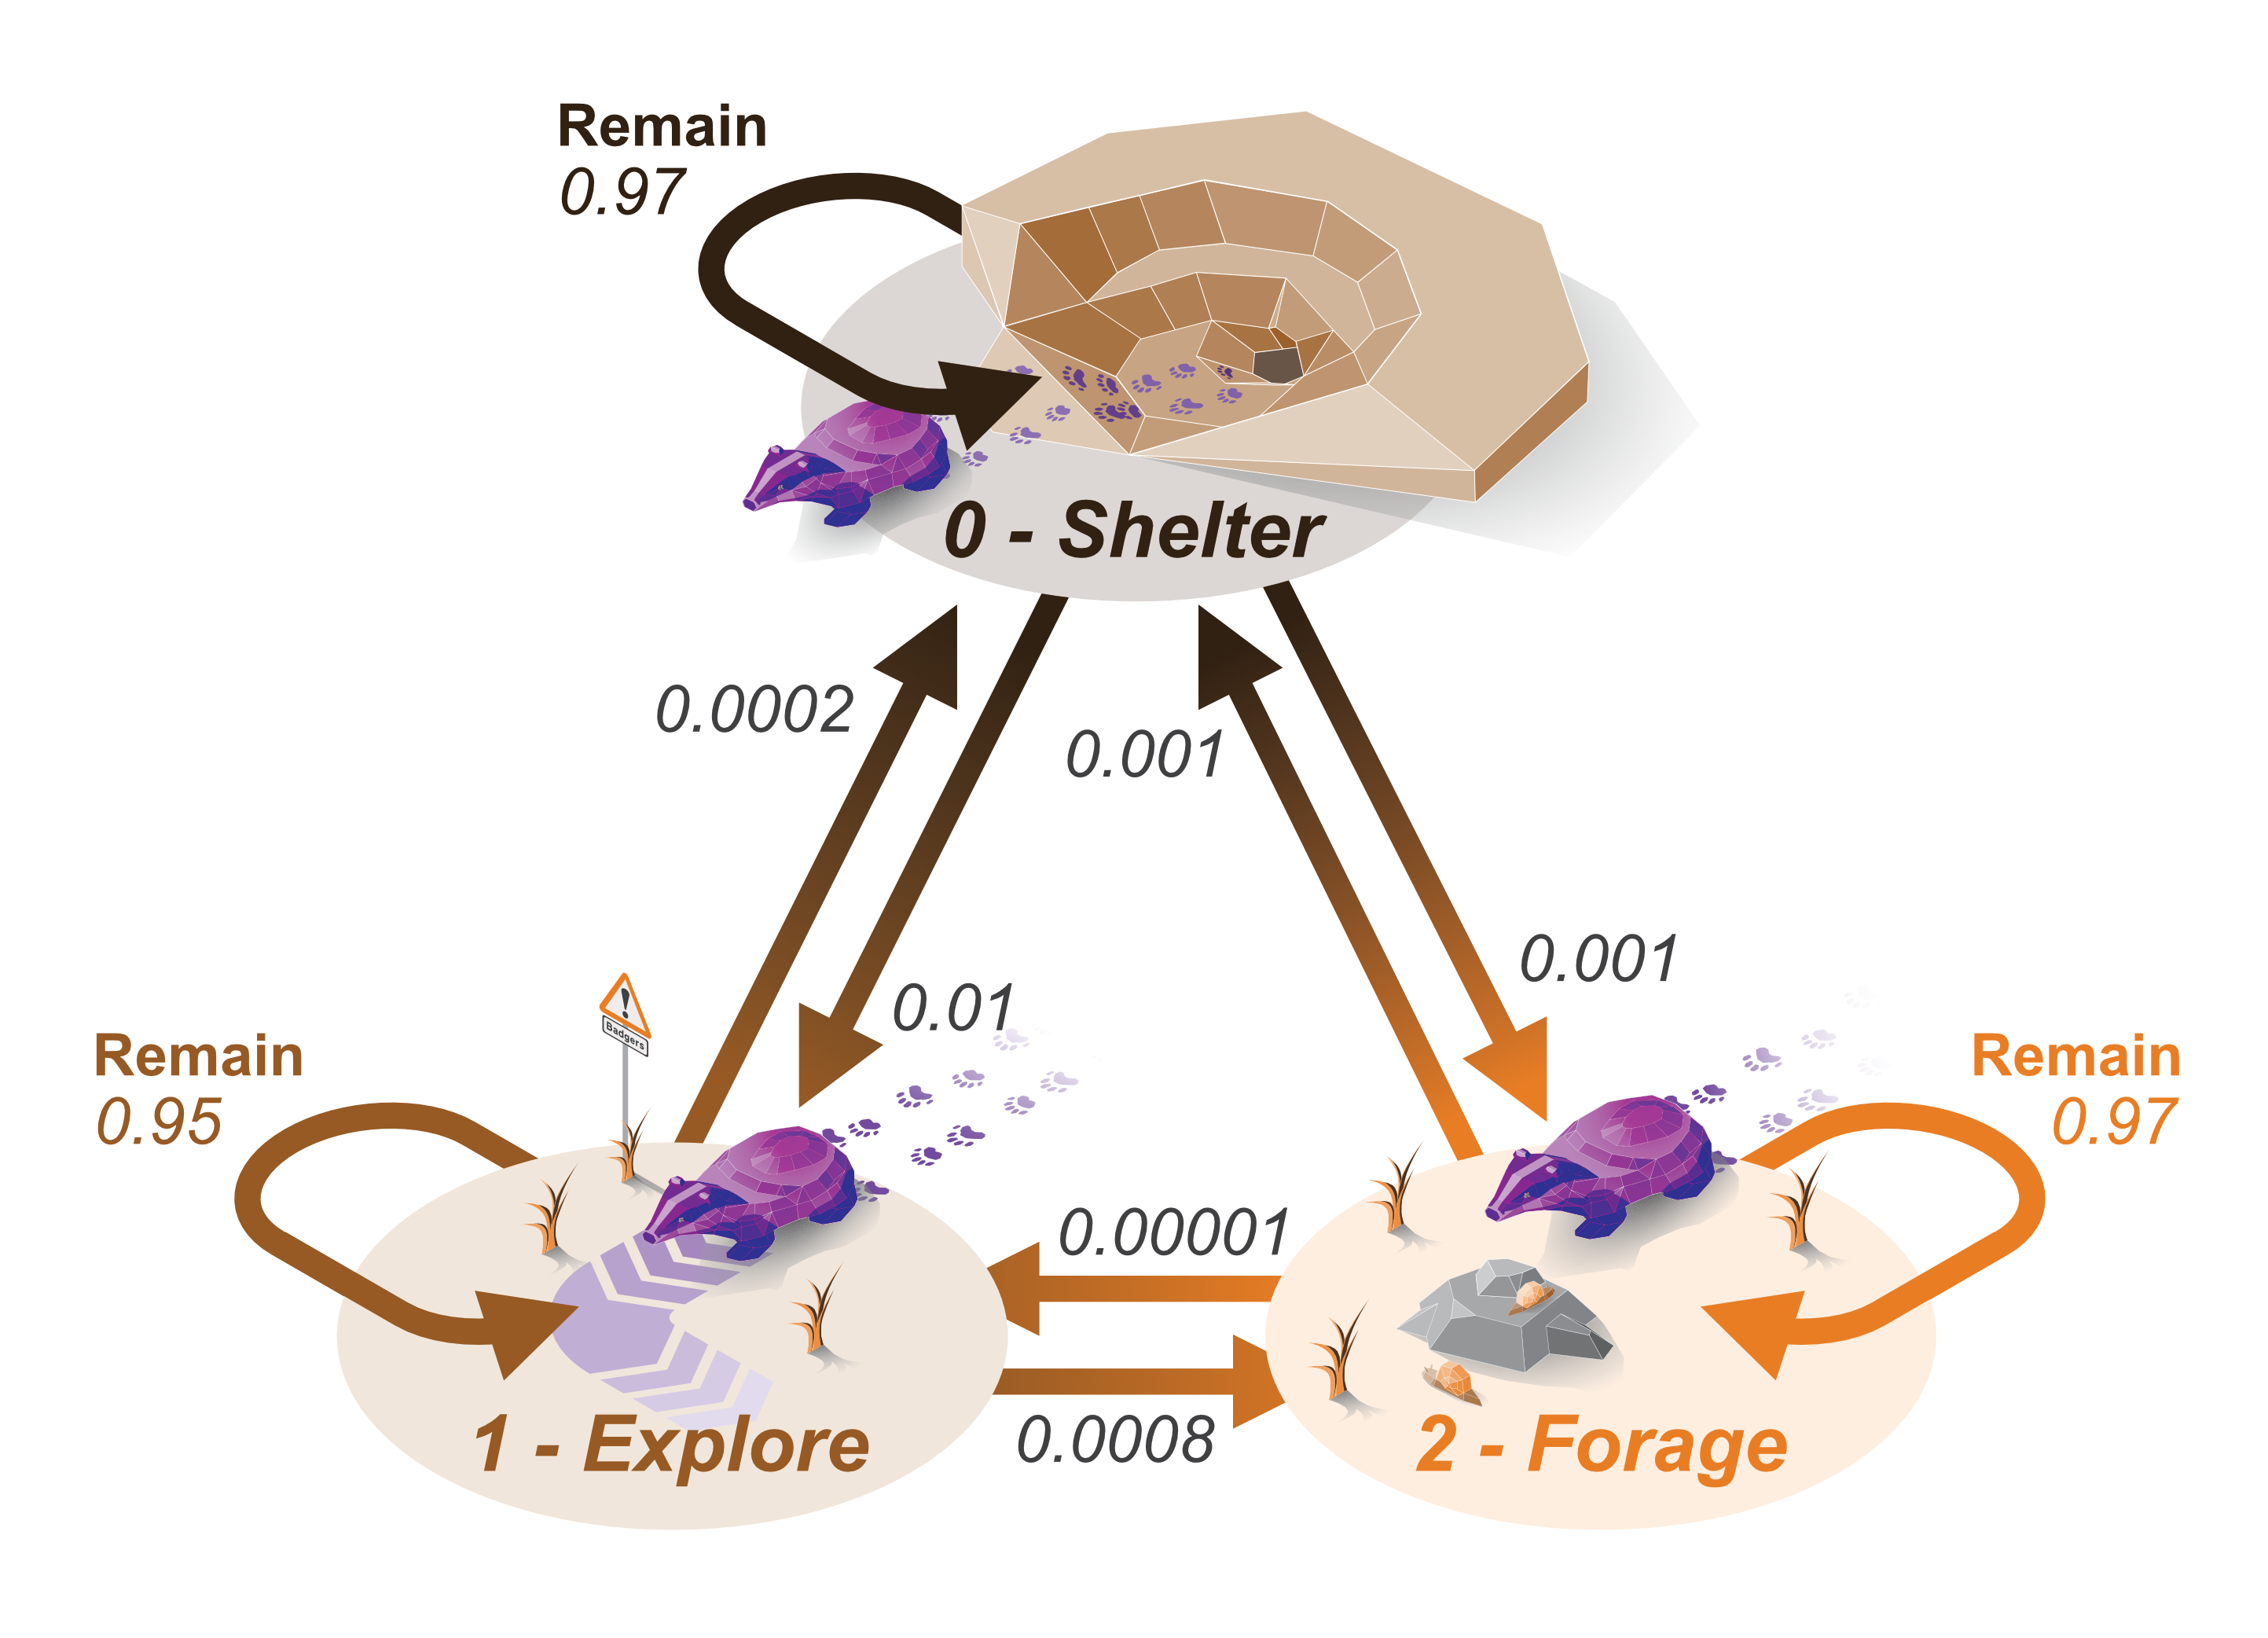
\includegraphics[width=0.8\linewidth]{../ext_figures/Tranistion Matrix Diagram} 

}

\caption{A diagram showing the transition probabilities between the three behavioural states. Remain values indicate the probabilities of the animal remaining in the same behavioural state. Values correspond directly to those in the transition matrix used as a simulation input.}\label{fig:transMatrixDiagram}
\end{figure}

\begin{verbatim}
##        b0      b1     b2
## b0 0.9700 0.01000 0.0010
## b1 0.0002 0.95000 0.0008
## b2 0.0010 0.00001 0.9900
\end{verbatim}

Animals' behaviour is frequently expressed via cycles, such as day/night or diel cycles (\citeproc{ref-rivera_rethinking_2022}{56}); therefore, we want the transition matrix to vary over time.
We describe a number of cycles (or waves) that can be applied to the core transition matrix impacting the probability of entering resting behaviour.
For example, a diel cycle can be expressed via a Sine wave with a frequency of 12 hours and an amplitude of 0.1.
At each time step we draw a value from the wave, and add that weighting (from -0.05 to 0.05) to the transition probability of entering resting state (row 1, column 1 of the matrix); therefore, the probability of resting will increase and decrease following the Sine wave at a approximately 12 hour activity pattern.
We can define as many cycles as needed, and they impact the resting probability additively.

When entering the resting state the animal will seek out a shelter site.
In the \emph{abmAnimalMovement} package, we can supply a number of shelter sites to simulate this need and create site fidelity.
As these shelter sites act as points of attraction for the animal for each rest, the animal occupies a consistent area, or something approximating a home range.
Home ranges are meant to represent areas in which the animal can source all resources required for a given life stage (\citeproc{ref-silva_autocorrelationinformed_2022}{44}).
The predefined and steady state of these shelter sites provides the stability we look for in a home range, as well as a means of predefining a level of site fidelity.
As the \emph{abmAnimalMovement} model can have multiple attraction (rest) sites supplied, we can simulate home ranges with unequal and behaviourally influenced space use.

\begin{figure}

{\centering 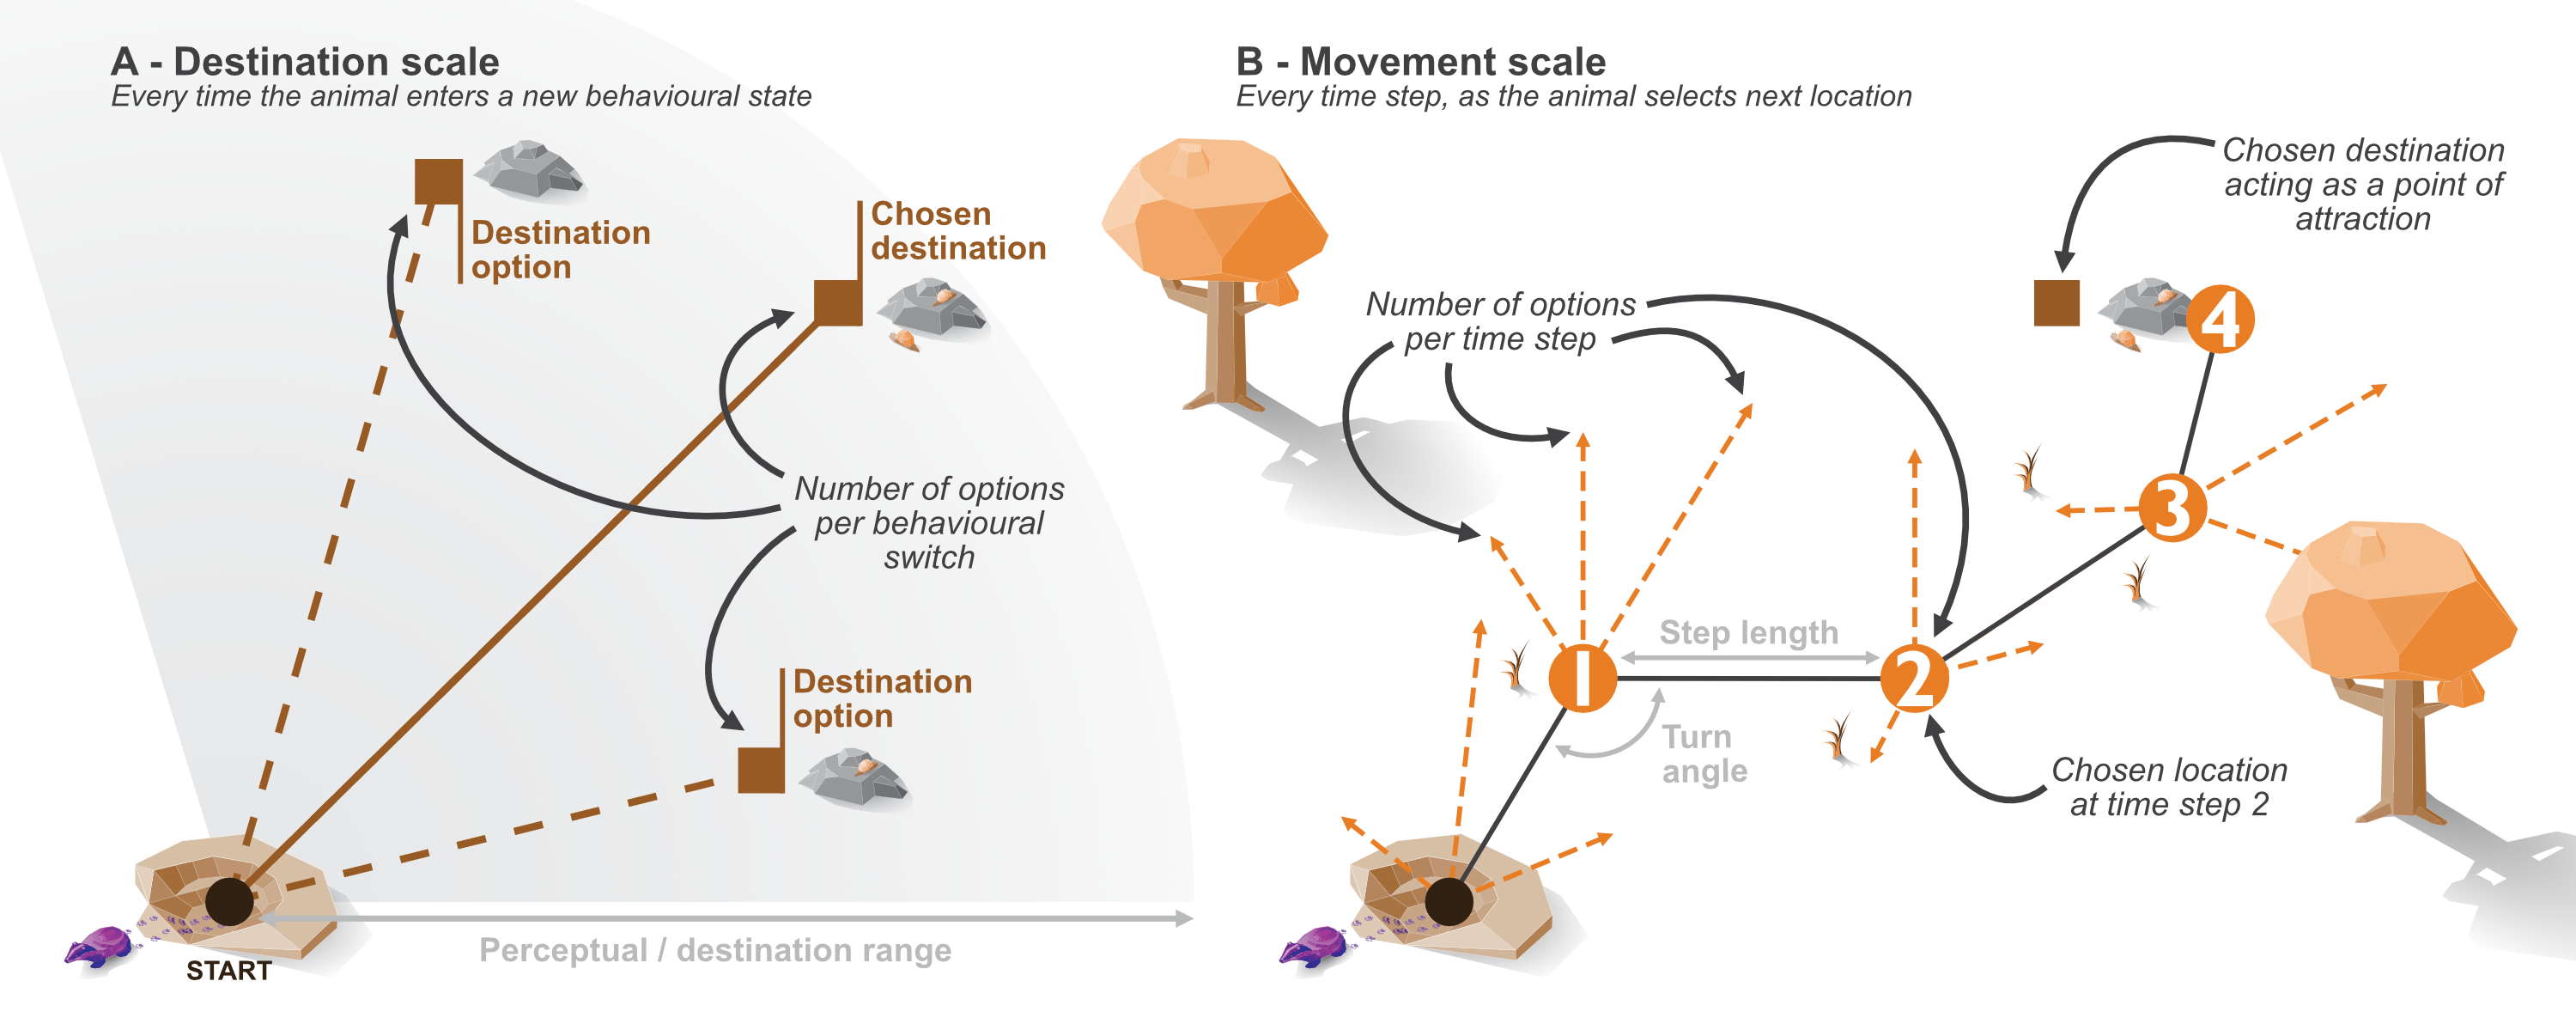
\includegraphics[width=0.85\linewidth]{../ext_figures/Simulation Process Diagram Static} 

}

\caption{A diagram showing the simulated animal's decision processes operating at two different time frames. A - the time frame of the destination choice, B - the time frame of movements at each time step.}\label{fig:walkDiagram}
\end{figure}

In addition to the predefined attraction to shelter sites, the \emph{abmAnimalMovement} package allows for a more dynamic attraction to areas of high resource quality.
Movements cannot be directly translated to animal preference; for example, habitat preference may miss key movement corridors (\citeproc{ref-Scharf2018}{57}); or the habitat decisions may occur at scales different to observed movement (\citeproc{ref-Bastille-Rousseau2017}{1}).
Therefore, the simulation required a mechanism that somewhat detaches the preference/choice for observed movements.
When entering foraging mode, the animal randomly selects foraging destinations as a point of attraction (but weighted towards areas of higher quality) (Figure \ref{fig:walkDiagram}).
This attraction impacts the movement choices made at each time step, with the animal more likely to choose (and therefore move to) options closer to the foraging destination.
Therefore, foraging destination choice operates on a different time frame to the movement and allows movements through low-quality foraging areas.
This presents a critical benefit of the simulation approach, as we define the internal state decision making process of the animal.
The two time frames also allow exploration of assumptions connecting observed movement choices to choices grounded in resource use, and whether downstream analyses can accurately recover a hidden decision making process.

At all times, the subsequent locations of the animal are impacted by a movement resistance matrix.
Differing values represent different environmental conditions that could change how easily/likely an animal is to use that area to move towards a destination.
For example, rivers or hard barriers within a landscape could present very high movement resistance and an animal would aim to avoid traversing them.
Alternatively, areas of lower movement resistance could aid movement, and potentially form movement corridors.
The movement matrix has values that describe the weighting of movement probability (lower values indicating a lower probability of entering a cell).
Whereas the resource environmental layer and shelter locations interact with destination/goal decisions, the movement resistance affects the step-by-step movement decisions.

The interplay between shelter sites, foraging quality, and movement resistance simulates the site fidelity required for home ranges, while allowing the environment to help shape the size and diffusion of that home range.
Simulating a more dynamic and messy array of movements can help test how far assumptions of uniform circular animal movement are practical.

\subsection{Generating three species}\label{generating-three-species}

To demonstrate the variation that movement ecology methods needs to wrangle, as well as the scope of movements the agent-based model can recreate, we provide three example species.
The examples cover a range of movement capacities, site fidelity, and resting/sheltering patterns.
Unlike alternative methods that are built to fit and simulate movements from existing data, our examples are loosely based on summary statistics from previous published results (cited below in each species section).
The choice of using species specific examples is intended to provide some biological context while demonstrating a range of simulation parametrisations.
Therefore, we are only interested in whether the simulated data returns the intended traits we are attempting to simulate for each example species (e.g., avoidance, site fidelity, expected step lengths).
We show one example via a more detailed walk-through (badger), and the other example parametrisations are included as uses cases at the end of the manuscript (vulture, king cobra).

\subsection{Primary example}\label{primary-example}

\subsubsection{Ecology and objectives - badger}\label{ecology-and-objectives---badger}

Our primary example is based on a badger.
Badgers occupy setts, in our example two home/shelter sites, to where they routinely return (\citeproc{ref-kowalczyk_daily_2006}{58},\citeproc{ref-feore_habitat_1999}{59}).
When not at the sett, the badger forages, and the foraging distances are impacted by resource position and movement capacity of the badger (i.e., how far can a badger feasibly travel for food from the sett).
The badger therefore expresses very high site fidelity, a range dictated by the spatial positioning of resources, and is subject to the movement resistance of the terrestrial environment.

We can draw on studies such as (\citeproc{ref-kowalczyk_daily_2006}{58}) and (\citeproc{ref-rosalino_activity_2005}{60}) to roughly gauge the speed of badgers (i.e., step length per minute).
How this speed differs between behaviours is more difficult to estimate from existing literature, but we can use (\citeproc{ref-kowalczyk_daily_2006}{58}) reported maximum speed to guide more direct movements (e.g., state 0 - sheltering and state 1 - exploring).
In particular (\citeproc{ref-kowalczyk_daily_2006}{58}) mentioned the heightened speeds moving from and to the setts.
We also want to allow the exploratory (state 1) movements to be great enough to occasionally exceed the normal home range or territory (\citeproc{ref-kelly_extra_2020}{61}).
We can draw on statements regarding maximum distance travelled in a night from papers such as (\citeproc{ref-rosalino_activity_2005}{60}), (\citeproc{ref-kowalczyk_daily_2006}{58}), and (\citeproc{ref-loureiro_path_2007}{62}) to approximate how distant foraging locations could be from a sett, while also confirming the nocturnal activity cycle for the badger.
For the example, we will consider badgers as fully nocturnal, and with active periods lasting for around 8 hours each night (\citeproc{ref-rosalino_activity_2005}{60},\citeproc{ref-magowan_dead-reckoning_2022}{63}).
The 8 hour active periods are not consistent throughout the year.
Badgers occupying temperate areas are impacted by seasonal shifts that modify daylight hours and available resources (\citeproc{ref-rosalino_activity_2005}{60},\citeproc{ref-magowan_dead-reckoning_2022}{63}).
Badger movements are also impacted by their territoriality, avoiding areas occupied by other badger groups, but also displaying occasional extra-territorial movements (\citeproc{ref-feore_habitat_1999}{59},\citeproc{ref-kelly_extra_2020}{61}).
This suggests a general, but not complete avoidance of areas occupied by other badger groups.

We can broadly summarise the badger ecology we want to parametrise as follows:

\begin{enumerate}
\def\labelenumi{\arabic{enumi}.}
\item
  Exhibits site fidelity via the use of two shelter sites (\citeproc{ref-kowalczyk_daily_2006}{58},\citeproc{ref-feore_habitat_1999}{59})
\item
  Movement speed approximated by summary statistics from previous studies (\citeproc{ref-kowalczyk_daily_2006}{58},\citeproc{ref-rosalino_activity_2005}{60}), while constrained by terrestrial environment and territoriality (\citeproc{ref-feore_habitat_1999}{59},\citeproc{ref-kelly_extra_2020}{61})
\item
  An 8-12 hour activity cycle, that shifts over the year (\citeproc{ref-rosalino_activity_2005}{60},\citeproc{ref-magowan_dead-reckoning_2022}{63})
\end{enumerate}

\subsection{Operation}\label{operation}

The \emph{abmAnimalMovement} package requires links to the \emph{Rcpp} (\textgreater= 1.0.8.3) (\citeproc{ref-Eddelbuettel_seamless_2011}{51}--\citeproc{ref-Eddelbuettel_extending_2018}{53}) and \emph{BH} (\textgreater= 1.78.0.0) packages (\citeproc{ref-Eddelbuettel_BH_2021}{64}), and therefore requires a version of \emph{R} \textgreater=3.5.0 (\citeproc{ref-R-base}{65}) (available from \href{https://www.r-project.org/}{www.r-project.org}).
Currently the \emph{abmAnimalMovement} package can be installed from Github using \texttt{install\_github} provided by the \emph{devtools} package (\citeproc{ref-Wickham_devtools_2021}{66}).

\subsection{Implemenation}\label{implemenation}

While only the \emph{abmAnimalMovement} package is required for running core simulations (\texttt{abm\_simulate} function), to generate, organise, and review the inputs and outputs of simulations, we make use of a number of \emph{R} packages.
An alternative simpler implementation with no dependencies is provided as a package vignette.

\begin{Shaded}
\begin{Highlighting}[]
\CommentTok{\# core package}
\FunctionTok{library}\NormalTok{(abmAnimalMovement)}
\CommentTok{\# data manipulation}
\FunctionTok{library}\NormalTok{(dplyr)}
\FunctionTok{library}\NormalTok{(reshape2)}
\CommentTok{\# visualisation}
\FunctionTok{library}\NormalTok{(ggplot2)}
\FunctionTok{library}\NormalTok{(ggforce)}
\FunctionTok{library}\NormalTok{(ggtext)}
\FunctionTok{library}\NormalTok{(ggridges)}
\FunctionTok{library}\NormalTok{(patchwork)}
\CommentTok{\# environmental matrix generation}
\FunctionTok{library}\NormalTok{(raster)}
\FunctionTok{library}\NormalTok{(NLMR)}
\end{Highlighting}
\end{Shaded}

We used \emph{R} v.4.4.2 (\citeproc{ref-R-base}{65}) via \emph{RStudio} v.2024.9.0.375 (\citeproc{ref-RStudioTeam2021}{67}), and used \emph{rmarkdown} v.2.29 (\citeproc{ref-R-rmarkdown}{68}--\citeproc{ref-rmarkdown2020}{70}), \emph{bookdown} v.0.42 (\citeproc{ref-bookdown2016}{71},\citeproc{ref-R-bookdown}{72}), \emph{tinytex} v.0.57 (\citeproc{ref-tinytex2019}{73},\citeproc{ref-R-tinytex}{74}), and \emph{knitr} v.1.49 (\citeproc{ref-knitr2015}{75}--\citeproc{ref-R-knitr}{77}) packages to generate type-set outputs.
We used the \emph{here} v.1.0.1 package (\citeproc{ref-R-here}{78}) to help with relative file path definition.
We used the \emph{dplyr} v.1.1.4 and \emph{reshape2} v.1.4.4 packages for data manipulation (\citeproc{ref-R-dplyr}{79},\citeproc{ref-reshape22007}{80}).
We used \emph{ggplot2} v.3.5.1 for creating figures (\citeproc{ref-R-ggplot2}{81},\citeproc{ref-ggplot22016}{82}), with the expansions: \emph{ggridges} v.0.5.6 (\citeproc{ref-R-ggridges}{83}), \emph{ggtext} v.0.1.2 (\citeproc{ref-R-ggtext}{84}), \emph{ggforce} v.0.4.2 (\citeproc{ref-R-ggforce}{85}), and \emph{patchwork} v.1.3.0 (\citeproc{ref-R-patchwork}{86}).
We used the \emph{raster} v.3.6.30 (\citeproc{ref-R-raster}{87}), \emph{sp} v.2.1.4 (\citeproc{ref-sp2013}{88}--\citeproc{ref-R-sp}{90}), and \emph{NLMR} v.1.1.1 (\citeproc{ref-NLMR2018}{91},\citeproc{ref-R-NLMR}{92}) for generating environmental matrices.

\subsubsection{Generating environmental matrices}\label{generating-environmental-matrices}

To ensure that the simulation completed during this example is repeatable, we set a seed.
For the sake of simplicity, the year the examples were written (2022) is used.

\begin{Shaded}
\begin{Highlighting}[]
\NormalTok{seed }\OtherTok{\textless{}{-}} \DecValTok{2022}
\FunctionTok{set.seed}\NormalTok{(seed)}
\end{Highlighting}
\end{Shaded}

Before starting to simulate animal movement, we needed to generate a landscape.
The landscapes in this case will take the form of matrices, where each cell is describing the quality of foraging, shelter, and movement ease.
The highest quality locations/cells are coded as 1, with quality decreasing as the values range down to 0.
The 1 to 0 quality values in each cell are later used to help the animal to choose how and where it moves throughout the landscape.
Depending on the behavioural state, the weighing of which matrix/layer used will change (e.g., when in a resting behavioural state the shelter site quality layer is used).

For most applications, a landscape would be known \emph{a priori}, but for this demonstration and testing of methods we use a selection of randomly generated landscape matrices (Figure \ref{fig:BADGERlayersFigure}), using the \emph{NLMR} package (neutral landscape models).

We used a Gaussian field with an autocorrelation range of 40, a magnitude of variation across the landscape of 5, a magnitude of variation in the scale of autocorrelation range of 0.2, and a mean of 0.5.
For foraging, we built on the Gaussian field already produced, allocating all values lower than 0.4 as 0 (i.e., no value for foraging), then normalising the remaining values between 0 and 1.

For a baseline movement resistance layer, we take the original Gaussian field and increase areas greater than 0.6 by 0.5 to allow areas of high resource quality to be easily accessible.
We also greatly increase the movement ease in ``edge'' habitat (+1), where values fall between 0.6 and 0.3.
Again we normalise between 0 and 1, where 1 are areas easily traversed.
The resulting environment is one with easily traversable edge areas, surrounding better quality foraging locations than can be moved into easily.

Shelter quality is intermediate; we increased weighting by +1 in areas where cell values were greater than 0.5 and lower than 0.7.
Thereby shelter sites are more likely to occur in the areas of higher foraging quality, but not in the core (i.e., \textgreater0.7), nor in the edge areas (\textless0.5).
This provides some balance between accessibility and proximity to resources.
The three matrices described provide a baseline for our examples, but can easily be modified for different scenarios (Figure \ref{fig:BADGERlayersFigure}).
To aid balancing, we keep values between 0 and 1; any numeric value can be used, but the simulation will interpret the values as relative weights when the animal is making decisions (Note: The current implementation of \texttt{cpp\_get\_values} that extracts values from the matrices during the simulation returns -99.9 weighting when presented with NA values; therefore, -99.9 serves as a lower limit to the matrix weighting values).

Once generated we supply the core simulation function (\texttt{abm\_simulate}) with each of these layers via the \texttt{shelteringMatrix}, \texttt{foragingMatrix}, and \texttt{movementMatrix} arguments.

\subsubsection{Animal parameters}\label{animal-parameters}

We predefine a suite of parameters describing the movement and behaviour characteristics of the animal (e.g., badger) based on summary statistics and general statements from previous research (\citeproc{ref-kowalczyk_daily_2006}{58}--\citeproc{ref-kelly_extra_2020}{61},\citeproc{ref-magowan_dead-reckoning_2022}{63}).
We store the parameters as objects we can later input into the \texttt{abm\_simulate} function.
We complete this process for three species; the badger values are displayed below, whereas the values for vulture and king cobra examples are provided at the end of the manuscript.

We parametrise shelter information in the following ways.
For the sett, we draw a two sets of coordinates from the shelter quality layer.
During the simulation the badger will randomly select a sett to return to each time it enters the resting behavioural state.
The choice of which sett to return to is weighted by the values supplied via the shelter quality environmental layer (Figure \ref{fig:BADGERlayersFigure}).
The coordinate data frame is provided to the core simulation function's \texttt{shelterLocations} argument.

The \texttt{shelterSize} argument describes the radius around the shelter locations within which the animal exhibits near stationary behaviour.
We specify the shelter size to be 8 m, meaning that when within 8 m of the selected shelter site the animal's possible step lengths are decreased 100-fold.
The shelter site size of 8 m allows for small movements near/within the sett during resting behaviour.

\begin{Shaded}
\begin{Highlighting}[]
\NormalTok{sampledShelters }\OtherTok{\textless{}{-}} \FunctionTok{sampleRandom}\NormalTok{(}\FunctionTok{raster}\NormalTok{(landscapeLayersList}\SpecialCharTok{$}\NormalTok{shelter), }\DecValTok{2}\NormalTok{,}
                                \AttributeTok{ext =} \FunctionTok{extent}\NormalTok{(}\FloatTok{0.45}\NormalTok{, }\FloatTok{0.65}\NormalTok{, }\FloatTok{0.45}\NormalTok{, }\FloatTok{0.65}\NormalTok{),}
                                \AttributeTok{rowcol =} \ConstantTok{TRUE}\NormalTok{)}

\NormalTok{BADGER\_shelterLocs }\OtherTok{\textless{}{-}} \FunctionTok{data.frame}\NormalTok{(}
  \StringTok{"x"} \OtherTok{=}\NormalTok{ sampledShelters[,}\DecValTok{2}\NormalTok{],}
  \StringTok{"y"} \OtherTok{=}\NormalTok{ sampledShelters[,}\DecValTok{1}\NormalTok{])}

\NormalTok{BADGER\_shelterSize }\OtherTok{\textless{}{-}} \DecValTok{8}
\end{Highlighting}
\end{Shaded}

\begin{figure}

{\centering 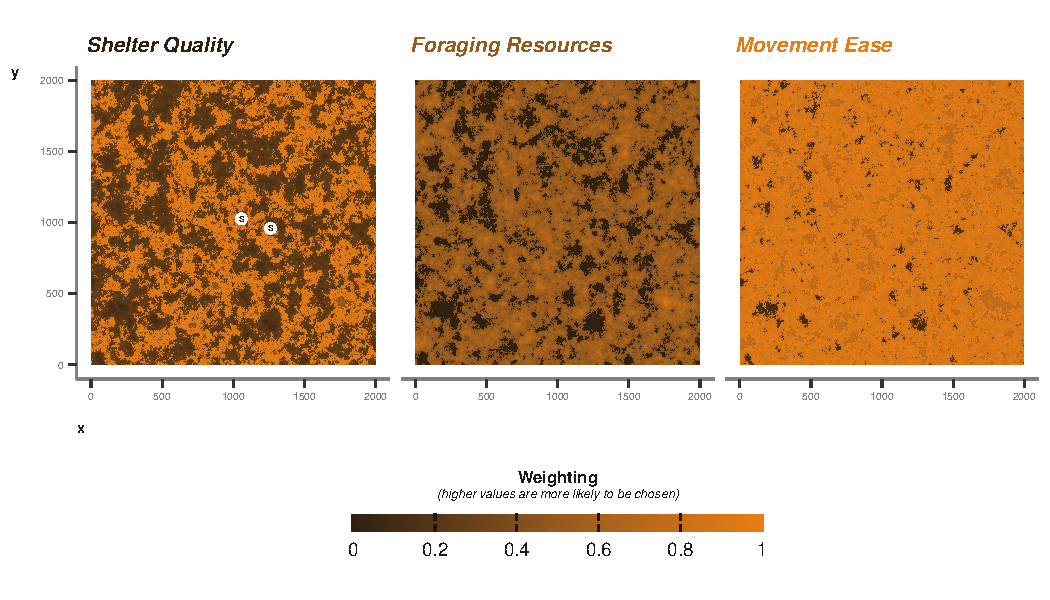
\includegraphics{Agent-based_model_walkthrough_files/figure-latex/BADGERlayersFigure-1} 

}

\caption{The three resulting landscape layers to be fed into the simulation for the badger example: shelter quality, foraging resources, movement ease.}\label{fig:BADGERlayersFigure}
\end{figure}

Badger movement is set via the definition of three pairs of Gamma and Von Misses distributions.
Each behavioural state is provided with a Gamma distribution to describe the step lengths between locations, and a Von Mises to describe the turn angles.
When combined, these two distributions provide the animal with a number of locations to choose from at each time step (Figure \ref{fig:walkDiagram}).
As we have three behavioural states, each movement parameter takes the form of a vector of length three.
The step lengths require predefined shape (k) and scale (\(\theta\)) parameters to describe the Gamma distributions, and we provide these to the simulate function via the \texttt{k\_step} and \texttt{s\_step} arguments.
For the turn angles we require the mean (\(\mu\)) and concentration (\(\kappa\)) to define the Von Mises distributions, and provide these via the \texttt{mu\_angle} and \texttt{k\_angle} arguments.

The perceptual range, in other words, where the badger decides to forage is set in a similar fashion.
Where \texttt{destinationRange} provides the shape (k) and scale (\(\theta\)) for the Gamma distribution describing distance of possible foraging locations, and \texttt{destinationDirection} provides the mean (\(\mu\)) and concentration (\(\kappa\)) the Von Mises distribution describing the angle at which those locations can fall (Figure \ref{fig:BADGERmoveCharFigure}).

We can also alter the strength of attraction to the foraging destinations.
At each time step, the animal is offered a number of location options to move to next time step.
The simulation calculates the distance between all options and the destination (i.e., a foraging location or shelter site), then normalises the distances between 0 and 1.
The normalised values serve as weighting to increase the chances the animal will move towards its destination.
We modify the weighting with the \texttt{destinationTransformation} and \texttt{destinationModifier} arguments.
The \texttt{destinationTransformation} allows for weightings to be transformed (where 0 = no transformation, 1 = weights are square-rooted, 2 = weights are squared).
Values supplied to \texttt{destinationModifier} apply a linear multiplicative effect to all the weightings.
When these weightings increase in value the animal will exhibit a stronger attraction and choose more direct movements to its current destination.

We also store a value ready for the \texttt{rescale\_step2cell} argument.
The rescale value is a simple means of adjusting the environment layers to fit with the scale/unit in which the step lengths are provided.
In this case, we treat each cell as 5m by 5m, thereby ensuring that our 2000x2000 matrix is sufficient for the badger to traverse without leaving.
The rescale value therefore allows high resolution movements on lower resolution environments, offering a crucial memory saving optimisation.

\begin{Shaded}
\begin{Highlighting}[]
\NormalTok{BADGER\_k\_step }\OtherTok{\textless{}{-}} \FunctionTok{c}\NormalTok{(}\FloatTok{0.3}\SpecialCharTok{*}\DecValTok{60}\NormalTok{, }\FloatTok{1.25}\SpecialCharTok{*}\DecValTok{60}\NormalTok{, }\FloatTok{0.25}\SpecialCharTok{*}\DecValTok{60}\NormalTok{)}
\NormalTok{BADGER\_s\_step }\OtherTok{\textless{}{-}} \FunctionTok{c}\NormalTok{(}\FloatTok{0.8}\NormalTok{, }\FloatTok{0.25}\NormalTok{, }\FloatTok{0.5}\NormalTok{)}
\NormalTok{BADGER\_mu\_angle }\OtherTok{\textless{}{-}} \FunctionTok{c}\NormalTok{(}\DecValTok{0}\NormalTok{, }\DecValTok{0}\NormalTok{, }\DecValTok{0}\NormalTok{)}
\NormalTok{BADGER\_k\_angle }\OtherTok{\textless{}{-}} \FunctionTok{c}\NormalTok{(}\FloatTok{0.6}\NormalTok{, }\FloatTok{0.99}\NormalTok{, }\FloatTok{0.6}\NormalTok{)}

\NormalTok{BADGER\_destinationRange }\OtherTok{\textless{}{-}} \FunctionTok{c}\NormalTok{(}\DecValTok{3}\NormalTok{, }\DecValTok{120}\NormalTok{)}
\NormalTok{BADGER\_destinationDirection }\OtherTok{\textless{}{-}} \FunctionTok{c}\NormalTok{(}\DecValTok{0}\NormalTok{, }\FloatTok{0.01}\NormalTok{)}
\NormalTok{BADGER\_destinationTransformation }\OtherTok{\textless{}{-}} \DecValTok{2}
\NormalTok{BADGER\_destinationModifier }\OtherTok{\textless{}{-}} \DecValTok{2}

\NormalTok{BADGER\_rescale }\OtherTok{\textless{}{-}} \DecValTok{5}
\end{Highlighting}
\end{Shaded}

The territoriality is not simulated directly via other individuals, instead we approximate it by supplying a number of point locations the badger will avoid.
An alternative way of simulating this behaviour would be to create areas of high movement resistance to prevent the badger from entering.
We provide a set of x, y coordinates of locations to be avoided.
Alongside the locations, we need to define how strongly the badger will avoid them using \texttt{avoidTransformation} (distance to point is weighting squared) and \texttt{avoidModifier} (distance to point is weighting multiplied by 4).
Both \texttt{avoidTransformation} and \texttt{avoidModifier} operate in the same way as the destination attraction arguments, but inverted; therefore, the avoidance behaviour will directly counteract the attraction to destination behaviour.

\begin{Shaded}
\begin{Highlighting}[]
\NormalTok{BADGER\_avoidLocs }\OtherTok{\textless{}{-}} \FunctionTok{data.frame}\NormalTok{(}
  \StringTok{"x"} \OtherTok{=} \FunctionTok{c}\NormalTok{(}\DecValTok{1205}\NormalTok{, }\DecValTok{1500}\NormalTok{, }\DecValTok{1165}\NormalTok{),}
  \StringTok{"y"} \OtherTok{=} \FunctionTok{c}\NormalTok{(}\DecValTok{980}\NormalTok{, }\DecValTok{1090}\NormalTok{, }\DecValTok{1250}\NormalTok{))}

\NormalTok{BADGER\_avoidTransformation }\OtherTok{\textless{}{-}} \DecValTok{2}
\NormalTok{BADGER\_avoidModifier }\OtherTok{\textless{}{-}} \DecValTok{4}
\end{Highlighting}
\end{Shaded}

We implement two cycles to capture the daily and seasonal cycles the badger experiences.
Both cycles are created by describing a Sine wave defined by its amplitude, midline, offset (\(\phi\)) and frequency (\(\tau\); via the \texttt{cycle\_draw} function).
The \texttt{abm\_simulate} function has two arguments for wave parameters: \texttt{rest\_Cycle} is a mandatory input to describe diel activity cycling, and \texttt{additional\_Cycles} to define any number of additive additional cycles.
For \texttt{rest\_Cycle} we will store a vector of length 4, with values defining the amplitude, midline, offset, and frequency in that order (Frequency is supplied in hours, i.e., 60 times the time step).
We set the amplitude to 0.12 and midline as 0, meaning the probability of resting will be modified by values ranging from -0.06 to 0.06 depending on the location in the wave.
Our badger example requires a 24 hour cycle where the probability of resting will peak and nadir, hence offset and frequency are set to 24 hours.
When combined with the base transition probability to rest, the above parametrisation creates a scenario of approximately 8 hour periods of activity every 24 hours.

To add a seasonal cycle we use \texttt{additional\_Cycles}.
We predefine a data frame where each row contains four elements describing the amplitude, midline, offset, and frequency.
Whereas our diel activity is defined by a 24 hour cycle, a seasonal cycle is 365 days and we shift the peak half a year (offset = 365/2).
The seasonal wave increases the probability of resting behaviour during a portion of the year, while not also overwhelming a relatively stable diel cycle (i.e., badger will sleep longer during one part of the year) as we have set a lower amplitude for the seasonal cycle (0.075).
A more extreme implementation of the second cycle could introduce hibernation behaviour.

We also pull forward the behaviour transition matrix we showed during the overview, and rename it so all simulation input objects have the \texttt{BADGER\_} prefix.

\begin{Shaded}
\begin{Highlighting}[]
\NormalTok{BADGER\_rest\_Cycle }\OtherTok{\textless{}{-}} \FunctionTok{c}\NormalTok{(}\FloatTok{0.12}\NormalTok{, }\DecValTok{0}\NormalTok{, }\DecValTok{24}\NormalTok{, }\DecValTok{24}\NormalTok{)}

\CommentTok{\# additional cycle}
\NormalTok{c0 }\OtherTok{\textless{}{-}} \FunctionTok{c}\NormalTok{(}\FloatTok{0.075}\NormalTok{, }\DecValTok{0}\NormalTok{, }\DecValTok{24}\SpecialCharTok{*}\NormalTok{ (}\DecValTok{365}\SpecialCharTok{/}\DecValTok{2}\NormalTok{), }\DecValTok{24}\SpecialCharTok{*} \DecValTok{365}\NormalTok{) }\CommentTok{\# seasonal}

\NormalTok{BADGER\_additional\_Cycles }\OtherTok{\textless{}{-}} \FunctionTok{rbind}\NormalTok{(c0)}
\NormalTok{BADGER\_additional\_Cycles}
\end{Highlighting}
\end{Shaded}

\begin{verbatim}
##     [,1] [,2] [,3] [,4]
## c0 0.075    0 4380 8760
\end{verbatim}

\begin{Shaded}
\begin{Highlighting}[]
\NormalTok{BADGER\_behaveMatrix }\OtherTok{\textless{}{-}}\NormalTok{ Default\_behaveMatrix}
\NormalTok{BADGER\_behaveMatrix}
\end{Highlighting}
\end{Shaded}

\begin{verbatim}
##        b0      b1     b2
## b0 0.9700 0.01000 0.0010
## b1 0.0002 0.95000 0.0008
## b2 0.0010 0.00001 0.9900
\end{verbatim}

\subsubsection{Running the simulation}\label{running-the-simulation}

We need to initially define a start location for our animal.
To introduce some more individual variation, we can randomly vary this starting location, but we restrict the start locations to be proximal to the centre of the environment.
For the simulation, we need a vector of length 2, where the first value is the x location, the second is y.

\begin{Shaded}
\begin{Highlighting}[]
\NormalTok{startLocation }\OtherTok{\textless{}{-}} \FunctionTok{sample}\NormalTok{(}\DecValTok{900}\SpecialCharTok{:}\DecValTok{1100}\NormalTok{, }\DecValTok{2}\NormalTok{, }\AttributeTok{replace =} \ConstantTok{TRUE}\NormalTok{)}
\end{Highlighting}
\end{Shaded}

We finally have some parameters that describe the scope and intensity of the simulation.
The length of the simulation is provided via the \texttt{timesteps} argument; in our examples we are operating under the assumption that one time step is equal to one minute.
Equally \texttt{timesteps} can be thought of as the number of movement choices simulated.
We also need to specify how many options will be drawn and considered by the animal at each time step.
The \texttt{options} argument is where this is input.
Similarly \texttt{des\_options} is where we specify the number of dynamically selected foraging attraction/destinations to choose from when it enters the foraging behaviour mode (state 1).

We can then call all our settings describing badger behaviour and movement settings we stored as objects previously, and run the simulation using \texttt{abm\_simulate} (Table \ref{tab:arguementTable}).

\begin{table}
\centering
\caption{\label{tab:arguementTable}Arguments fed into main \texttt{abm\_simulate} function. Arguements are the terms used in teh function, the inputs are the R objects created during this example, the descriptions provide a brief overview of what the arguement is configuring.}
\centering
\fontsize{10}{12}\selectfont
\begin{tabular}[t]{>{\raggedright\arraybackslash}p{11em}>{\raggedright\arraybackslash}p{16em}>{\raggedright\arraybackslash}p{22em}}
\toprule
Argument & Input & Description\\
\midrule
start & startLocation & a data frame with x and y coordinates\\
timesteps & simSteps & an integer describing the length of the simulation\\
des\_options & 10 & an integer describing the number of foraging destination options an animal is offered\\
options & 12 & an integer describing the number of movement options an animal is offered\\
shelterLocations & BADGER\_shelterLocs & a data frame providing x and y coordinates of the shelter locations\\
\addlinespace
shelterSize & BADGER\_shelterSize & a value describing the radius around shelter sites that movement step lengths are reduced\\
avoidPoints & BADGER\_avoidLocs & a data frame providing x and y coordinates of the avoidance locations\\
destinationRange & BADGER\_destinationRange & a numeric vector of length two that contains the shape and scale values that describe the Gamma distribution for potential foraging destinations\\
destinationDirection & BADGER\_destinationDirection & a numeric vector of length two that contains the mean and concentration values that describe the Von Mises distribution for potential foraging destinations\\
destinationTransformation & BADGER\_destinationTransformation & a value to choose the type of transformation applied to the animal's attraction to a chosen destination\\
\addlinespace
destinationModifier & BADGER\_destinationModifier & a value modifying the animal's attraction to a chosen destination\\
avoidTransformation & BADGER\_avoidTransformation & a value to chose the type of transformation applied to the animal's avoidance to avoidance locations\\
avoidModifier & BADGER\_avoidModifier & a value modifying the animal's avoidance of avoidance locations\\
k\_step & BADGER\_k\_step & a vector of three numbers describing the three behavioural states' Gamma distributions' shape parameter for step lengths\\
s\_step & BADGER\_s\_step & a vector of three numbers describing the three behavioural states' Gamma distributions' scale parameter for step lengths\\
\addlinespace
mu\_angle & BADGER\_mu\_angle & a vector of three numbers describing the three behavioural states' Von Mises distributions' mean parameter for turn angles\\
k\_angle & BADGER\_k\_angle & a vector of three numbers describing the three behavioural states' Von Mises distributions' concentration parameter for turn angles\\
rescale\_step2cell & BADGER\_rescale & a numeric value to specify the size of the environmental matrices cells\\
behave\_Tmat & BADGER\_behaveMatrix & a 3x3 numeric matrix describing the transition probabilities between the three behavioural states\\
rest\_Cycle & BADGER\_rest\_Cycle & a vector length 4 for amplitude, midline, offset and frequency to define the resting/active cycle\\
\addlinespace
additional\_Cycles & BADGER\_additional\_Cycles & a data.frame 4 columns wide for amplitude, midline, offset and frequency to define any additional activity cycles, where each row is another cycle\\
shelteringMatrix & BADGER\_shelter & three arguments for the three matrices describing the landscape the simulated animal occupies\\
foragingMatrix & BADGER\_forage & \\
movementMatrix & BADGER\_move & \\
\bottomrule
\end{tabular}
\end{table}

\section{Results}\label{results}

\subsection{Output format}\label{output-format}

The simulation function (\texttt{abm\_simulate}) outputs a list containing: (1) a dataframe of realised movements, (2) a dataframe of options the animal had available, and (3) a list of the inputs used to simulate the movement.
The realised movement dataframe (\texttt{locations}) describes all realised locations the animal occupied, step length information, behavioural state, and current point of attraction, where each row is equal to a time step.
Note the simulation is scale agnostic, so each row can represent a different time step to the example.
Other than the lack of timestamps and location error, the format largely mirrors a typical movement dataset.
Our example is minute by minute; changing the time step would require a reparametrisation of step length and behavioural transition probabilities.
The \texttt{options} dataframe describes all the options available to the animal over the entire simulation duration, where each row is equal to an option repeated for each time step.

\subsection{Outputs review}\label{outputs-review}

Once simulated, we can review the movement characteristics of the three species.
The simplest to examine is the movement speeds or step lengths.
During the simulation parametrisation we provided rescale values for the size of the cells describing environmental information (see \texttt{rescale\_step2cell} argument).
The simulated movement will return the scaled values, so to plot something comparable to the input values, we must rescale the simulated step lengths.

\begin{figure}

{\centering 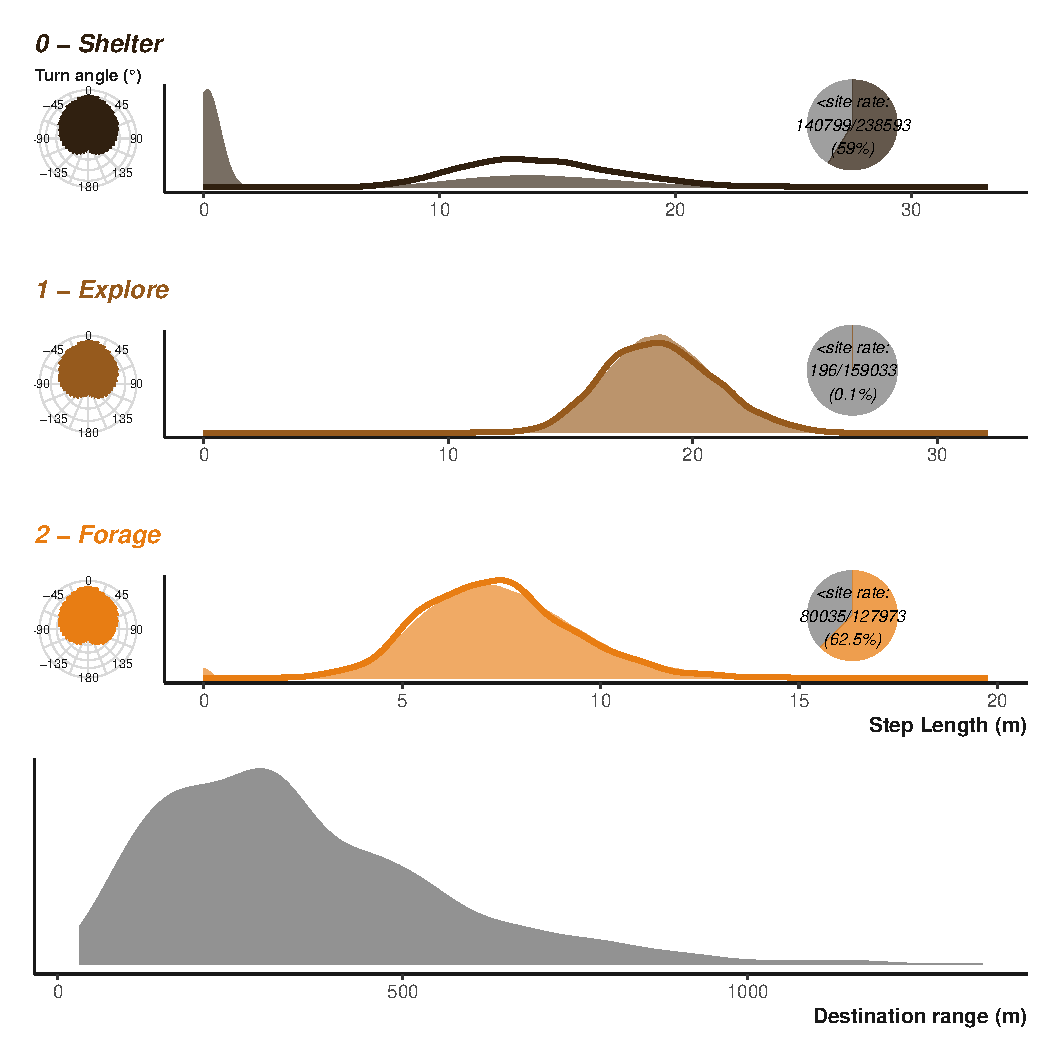
\includegraphics{Agent-based_model_walkthrough_files/figure-latex/BADGERmoveCharFigure-1} 

}

\caption{The distribution of step lengths used during the badger simulation example. Parametrising distributions are shown as solid areas using the same shape and scale parameters used as input into the simulation function. The lower plot shows the distribution used to generate potential foraging destinations. The realised resulting simulated step lengths (scaled to the input units) are shown by the solid lines. The realised resulting turn angles are shown in left hand sub-plots. Inset pie charts show the number of step lengths that were below the shelter site size. Note that x axis is not consistent between the three plots.}\label{fig:BADGERmoveCharFigure}
\end{figure}

We can compare the simulation's inputs displayed in to the simulated/observed outputs displayed in Figure \ref{fig:BADGERmoveCharFigure} and see that they largely agree as expected.
The turn angles are more variable, as the destination decisions and attraction to locations heavily influence the distribution overriding the initial parametrisation of the Von Mises distribution.
Figure \ref{fig:VULTUREmoveCharFigure} and Figure \ref{fig:KINGCOBRAmoveCharFigure} in the use cases section show the outputs for vulture and king cobra simulations.

We can review how the movements appear in space.
With the badger example, the impact of the avoidance points is clearly visible (Figure \ref{fig:mapsFigure}a), whereas the lack of or weaker avoidance in vulture (Figure \ref{fig:mapsFigure}b) and king cobra (Figure \ref{fig:mapsFigure}c) makes the avoidance less influential.
The vulture's movements and chosen foraging locations are largely to the east, demonstrating the impact of the underlying foraging quality environmental layer.
The king cobra plot shows the impact of a near impermeable barrier truncating the southward movements.

\begin{figure}

{\centering 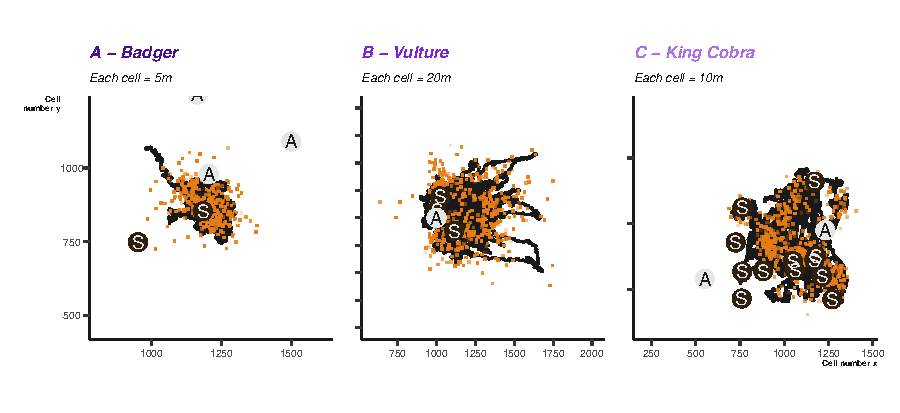
\includegraphics{Agent-based_model_walkthrough_files/figure-latex/mapsFigure-1} 

}

\caption{The observed locations of the three simulated species (A - Badger, B - Vulture, C - King Cobra). Black points show the observed location at each time step. The orange squares show the dynamically selected foraging destinations. Circles with an interior S show the shelter site locations, and cricles with an interior A show the avoidance points. Note that the size represented by each unit on the x and y axis differs depending on the species.}\label{fig:mapsFigure}
\end{figure}

\begin{figure}

{\centering 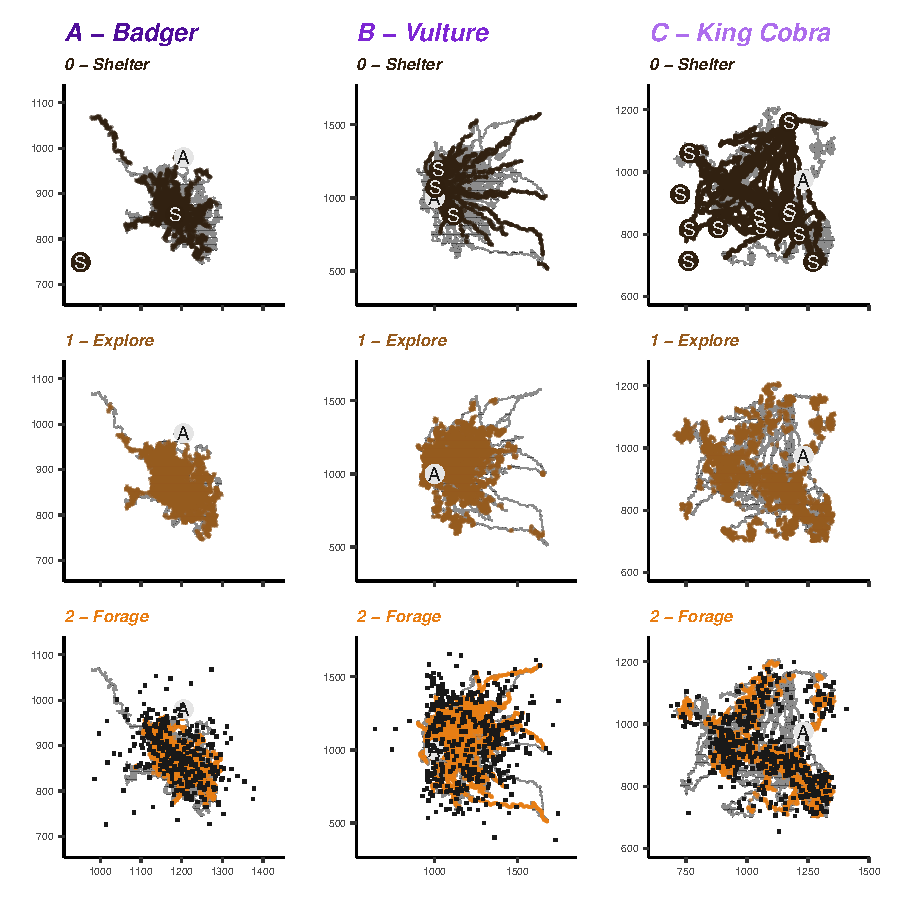
\includegraphics{Agent-based_model_walkthrough_files/figure-latex/oneMonthMapFigure-1} 

}

\caption{The observed locations of the three simulated species (A - Badger, B - Vulture, C - King Cobra) over the first month of time steps. Grey path shows the overall movement during that month, overlaid points indicate where the animal was in a given behavioural mode. Circles with an interior S show the shelter site locations, and cricles with an interior A show the avoidance points, black squares show the dynamically selected foraging destinations. Note that the size represented by each unit on the x and y axis differs depending on the species.}\label{fig:oneMonthMapFigure}
\end{figure}

The activity cycles and the timing of behavioural shifts is a key component in the simulations.
We can examine that the predefined cycles result in expected patterns.
A year of data makes observing all but the broadest cycles difficult, so in Figure \ref{fig:cycleFigure} we can look at several months of data as well as the daily cycle.
Badger and vulture daily cycles are largely the same (Figure \ref{fig:cycleFigure}a \& b), with a consistent daily activity cycle differing only slightly in the time spent active and balance between shifts from sheltering to foraging and exploring.
Some of the differences are a result of the different behavioural transition matrix provided to simulated the two species, where both had different baseline probabilities of shifting between behavioural states.
By contrast, the king cobra example demonstrates the interaction between the daily and weekly cycles (Figure \ref{fig:cycleFigure}).
We can see intermittently extended sheltering periods, punctuated by short exploratory or foraging bouts.

\begin{figure}

{\centering 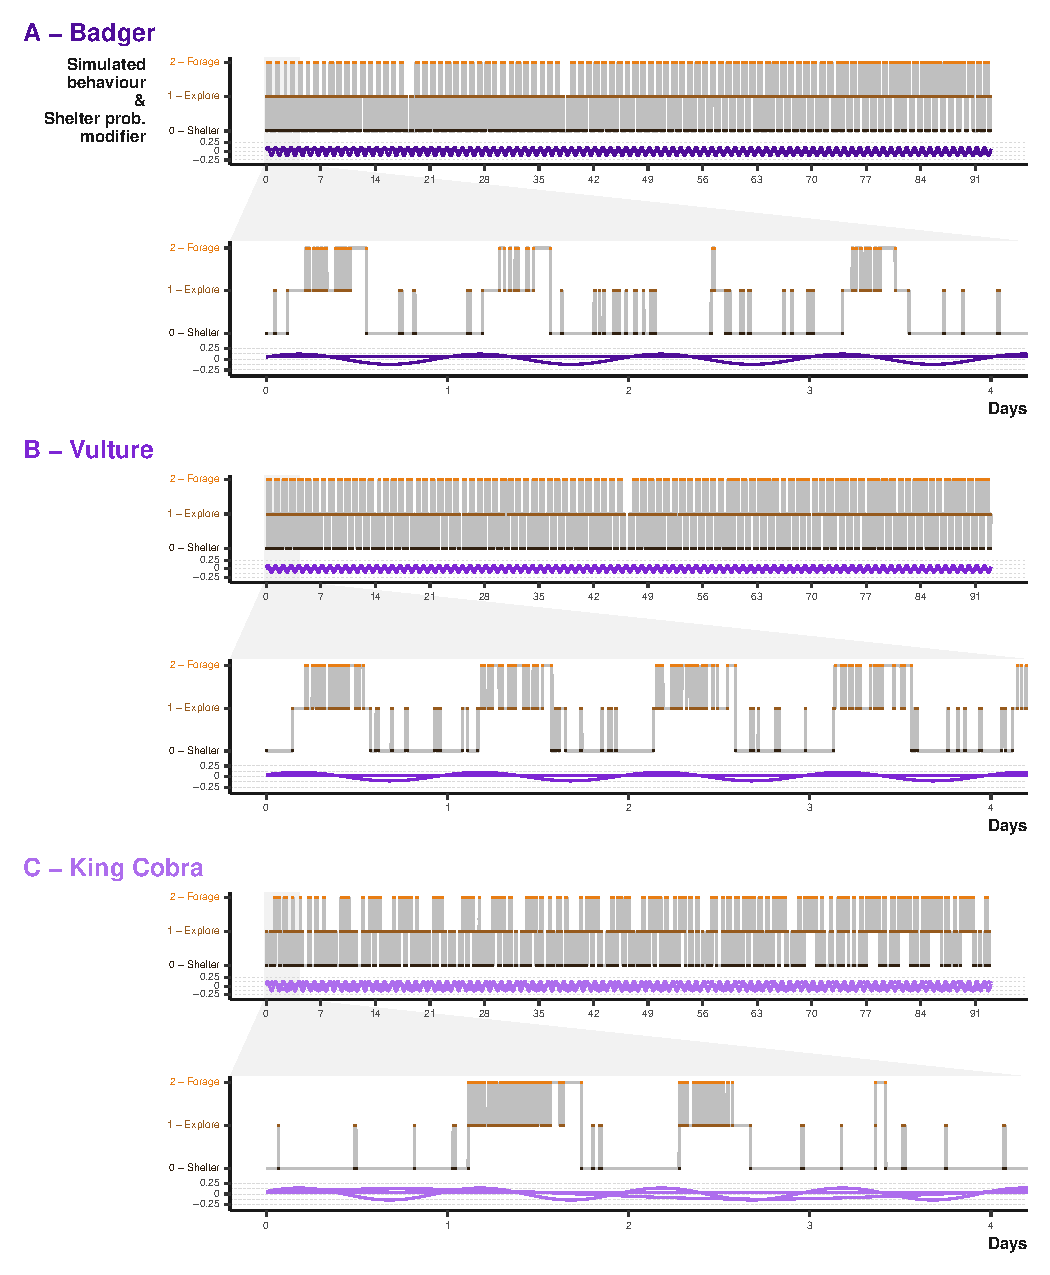
\includegraphics{Agent-based_model_walkthrough_files/figure-latex/cycleFigure-1} 

}

\caption{The observered (top half) and parametrised activty cycles (bottom half) governing sheltering behaviour in the three example species (A - Badger, B - Vulture, C - King Cobra). Point colour and position describe the behavioural state at each simulated time step, whereas the purple waves indicated the input values. Note that the input waves acting on the simulated animal in conjunction with the beahvioural transition matrix.}\label{fig:cycleFigure}
\end{figure}

At the daily and monthly scale, we cannot see the impact of the broad scale seasonal cycles.
Instead we can look at the percentage of time steps per day the animal was in sheltering behaviour (Figure \ref{fig:cycleSeasonalFigure}).
Again the badger and vulture sheltering rates are similar, differing in intensity, but with both demonstrating a seasonal decrease in the middle of the simulation.
The king cobra cycles reveal a decrease in the number of days spent entirely sheltering and an overall impression that the seasonal cycle is less influential (as it is only one of three activity cycles).

\begin{figure}

{\centering 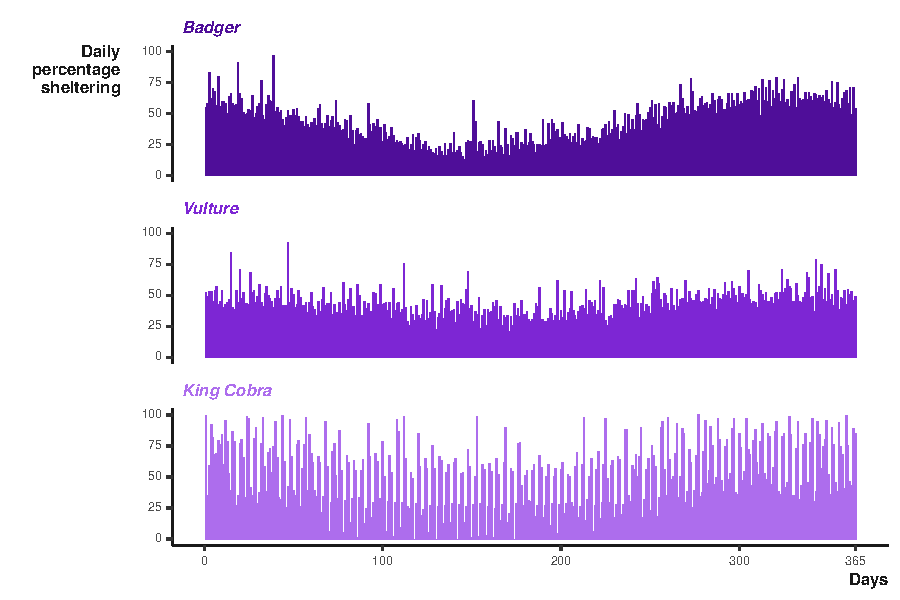
\includegraphics{Agent-based_model_walkthrough_files/figure-latex/cycleSeasonalFigure-1} 

}

\caption{The percentage of time steps spent in state 0 - resting per day, and how it varies over the entire simulated year.}\label{fig:cycleSeasonalFigure}
\end{figure}

\section{Discussion}\label{discussion}

Animal movement datasets are complex and require a suite of analytical approaches to tackle satisfactorily.
Efforts to develop new, and test existing, analyses would be aided by access to a range of diverse datasets.
While \emph{ideal} simulations often accompany new analysis methods and provide superb validation for the method in question, reaffirming the method's robustness and pushing them to new limits with a messier, more stochastic, simulation approach could greatly strengthen our confidence in results.
The \emph{abmAnimalMovement} package provides an independent route to test new methods that covers a range of interacting movement features, not necessarily directly tied to a single analytical method.

By including a range of features linked to movement and behaviour, the \emph{abmAnimalMovement} package can be implemented to investigate a suite of questions commonly asked of movement data --from habitat selection, to behaviour detection (for examples of common themes see \citeproc{ref-joo_recent_2022}{13}).
While some of the features can appear simplistic, there remains ample flexibility to simulate a wide range of useful scenarios.
For example, we conceptualise the three movement states as sheltering, exploring, and foraging.
However, only several aspects are immutable: one state exhibits site fidelity (state 0), one state is free from all attraction (state 1), and one state is driven by an underlying environmental layer (state 2).

The \emph{abmAnimalMovement} package has an advantage over data-driven simulation methods in scenarios where data are scarce, as much of the animal world is untracked (\citeproc{ref-joo_recent_2022}{13},\citeproc{ref-crane_lots_2021}{25}).
For the untracked animals, we may be limited to basic information of speed, activity, and resources, or such information may even need to be inferred from ecologically similar species.
In such data starved situations, the \emph{abmAnimalMovement} package's low computational cost and minimal data requirements allows for a large number of alternative parametrisations to be explored.
Via the explorations of different parametrisations researchers can help build a picture of the study and analysis methods best suited for their questions, with the opportunity to test those analyses on synthetic simulated data.

In cases where data cannot be shared (e.g.~due to concerns over species sensitivity), using a synthetic dataset could allow researchers to provide peer reviewers a dataset to test and error-check analysis code (\citeproc{ref-Quintana2020}{93}).
Providing data is a key component to ensuring computational reproducibility (\citeproc{ref-Gerstner2017}{94}), and synthetic datasets provide an avenue to limit the reproducibility loss from data sharing restrictions.
Additionally, such synthetic datasets could be integrated into preregistration as a means of demonstrating the validity of an analysis plan prior to undertaking a study.

Producing a range of simulated datasets that cover alternate scenarios may present researchers opportunities to test real data against a null model.
For example, researchers looking to investigate whether an animal was avoiding a certain landscape feature could calibrate a number of simulations covering a range of differing avoidance strengths.
The simulated results could then be compared to the real data to gauge how different the real data was from simulations exhibiting zero avoidance (i.e., a null model scenario).
This approach could complement current analysis methods, akin to sensitivity analysis.

\subsection{Future directions}\label{future-directions}

The \emph{abmAnimalMovement} package provides adequate functionality to simulate a range of scenarios and movements.
However, there are several aspects that will bear updating in future versions.

\begin{enumerate}
\def\labelenumi{\arabic{enumi}.}
\item
  Dynamic state 0. While state 0 and the steady state of the attraction locations is key to simulating range stability (i.e., home range), there may be scenarios where this stability is not desired.
  For example, when simulating dispersal behaviour of juvenile or sub-adult animals there may be a desire to have shelter site dynamically chosen for a time.
  Currently such behaviour could be simulated, but it would require the dispersal to occur immediately, and the dispersal destination to be predefined (i.e., the sites for state 0 attraction).
  Therefore, in the current state the package may be limited in its ability to help predict possible dispersal destinations, but potentially capable of informing dispersal routes.
\item
  Autocorrelated speed. We may need to improve the autocorrelation of the animal's speed.
  Currently the speeds are non-independent based on the behavioural mode of the animal.
  The need to implement a more aggressive movement momentum/autocorrelative structure may be felt more acutely at different time frames, and for animals with a great variation in step lengths (i.e., a larger \(\theta\) for the Gamma distribution).
  Explorations of simulated data using methods that measure autocorrelation in animal speed will reveal how much of a priority this should be.
\item
  Dynamic environment. All the environmental matrices are static; currently there is no system to update values during the simulation.
  This prevents shifts in the landscape such as seasonal variation in resources, or the development of trails.
  Currently, the closest solution is to run multiple simulations where the end location of simulation\textsubscript{1} is the start location for simulation\textsubscript{2}, where simulation\textsubscript{2} is provided with a new season-appropriate resource layer.
  This solution would be inadequate for trail development, as trail development would require a system within the simulation to update previously used cells for the animal at each time step.
\end{enumerate}

\subsection{Use cases}\label{use-cases}

This section provides alternative parametrisations for the secondary examples to better demonstrate the range of movement types and scenarios the \emph{abmAnimalMovement} package can replicate.
We provide example implementations of vulture and king cobra -like movement.

\subsubsection{Ecology and objectives - vulture}\label{ecology-and-objectives---vulture}

Unlike badgers and other terrestrially moving animals, vultures can move great distances with minimal obstruction (Figure \ref{fig:VULTURElayersFigure}).
Vultures can also move greater distances more rapidly (\citeproc{ref-hribsek_first_2021}{95}), resulting in a more variable and distribution of step lengths (\citeproc{ref-garcia-jimenez_drivers_2018}{96}--\citeproc{ref-subedi_spatial_2020}{98}) (Figure \ref{fig:VULTUREmoveCharFigure}).

Similar to badgers, vultures exhibit significant site fidelity, re-using roosting and nesting sites (\citeproc{ref-bracis_revisitation_2018}{99}).
Such shelter sites could be predefined; for example, if shelter sites were known \emph{a priori} discovered via the capture and tagging of animals, which in the case of birds is more likely.

Vultures also offer an opportunity to demonstrate how the underlying resource availability impacts the movements of animals.
In the case of vultures, their moments have been seen to follow carcasses, creating starkly contrasting areas where vultures will and will not travel (\citeproc{ref-arrondo_invisible_2018}{9}) (Figure \ref{fig:VULTURElayersFigure}).

Vultures have a very similar cycle pattern to the badgers (just inverted), one defined by a standard 12 hours of activity during the day, and 12 hours of increased resting behaviour during the night.
The importance of simulating such cycles is made clear by vultures studies demonstrating that day-night cycles can impact rates of location collection (\citeproc{ref-silva_seasonal_2017}{100}).
How the the animals' activity cycle and the probability of collected data interact could be a key consideration for some research questions.
Again, similar to badgers we would expect seasonal shifts in the form of an increase and decrease in activity depending on the time of year (\citeproc{ref-hribsek_first_2021}{95},\citeproc{ref-garcia-jimenez_drivers_2018}{96},\citeproc{ref-peshev_new_2021}{101}).

We can broadly summarise the vulture ecology we want to parametrise as follows:

\begin{enumerate}
\def\labelenumi{\arabic{enumi}.}
\item
  Medium site fidelity via the use of multiple roosting/resting sites (\citeproc{ref-bracis_revisitation_2018}{99})
\item
  Movement speed approximated by summary statistics from previous studies (\citeproc{ref-hribsek_first_2021}{95}--\citeproc{ref-subedi_spatial_2020}{98}), with minimal landscape derived resistance
\item
  A 8-12 hour activity cycle, that shifts over the year
\end{enumerate}

\subsubsection{Ecology and objectives - king cobra}\label{ecology-and-objectives---king-cobra}

Whereas the previous two species have a very limited or single shelter sites, king cobras make use of a wider range of shelter sites distributed more widely over their home ranges (\citeproc{ref-Marshall2018}{102},\citeproc{ref-marshall_no_2020}{103}).
These sites can also be larger, comprising of burrow systems or rock complexes.

What more dramatically sets king cobras, and other snakes, apart is a vastly differing rest-forage cycle.
While snakes still exhibit a diel cycle, the intermittent depredation of large prey items and the time required sheltering to digest large meals results in a second broader activity cycle operating over a more widely observed diel cycle (\citeproc{ref-marshall_no_2020}{103}--\citeproc{ref-Siers2018}{106}).
We can conceptualise this pattern as two additive cycles, one that will describe the daily activity cycle, and a second that describes the foraging and digestion cycle.
Seasonality also impacts king cobra activity.
As king cobras occupy tropical regions, the seasonality they experience is not as pronounced as the badger or vulture examples.
Overall king cobras have three activity cycles acting on three different scales.

In this example we can also demonstrate the movement resistance dramatically impacting movement possibilities.
King cobra movement can be limited by roads (\citeproc{ref-jones_how_2022}{107},\citeproc{ref-Marshall2018b}{108}), where unless provided with crossing structures king cobras are vulnerable to vehicle hits (Figure \ref{fig:KINGCOBRAlayersFigure}).
In addition to roads presenting linear barriers across the landscape, king cobras face persecution when near or in human settlements (\citeproc{ref-Marshall2018b}{108},\citeproc{ref-Shankar2013}{109}).
Despite the risks, avoidance of such areas appears weak.

Finally, king cobra movement characteristics will be dramatically reduced compared to the vulture's, but with similar shape to the badger with greater variability (Figure \ref{fig:KINGCOBRAmoveCharFigure}) as king cobras are known to range over large areas (\citeproc{ref-Marshall2018}{102},\citeproc{ref-marshall_no_2020}{103},\citeproc{ref-Silva2018}{110}).

We can broadly summarise the king cobra ecology we want to parametrise as follows:

\begin{enumerate}
\def\labelenumi{\arabic{enumi}.}
\item
  Lower site fidelity via the use of many shelter sites (\citeproc{ref-Marshall2018}{102},\citeproc{ref-marshall_no_2020}{103})
\item
  Movement speed approximated by summary statistics from previous studies (\citeproc{ref-Marshall2018}{102},\citeproc{ref-marshall_no_2020}{103},\citeproc{ref-Silva2018}{110}), with examples of very high landscape derived resistance (\citeproc{ref-jones_how_2022}{107},\citeproc{ref-Marshall2018b}{108})
\item
  A 8-12 hour activity cycle, with a approximately weekly forage-digest cycle, and weak seasonality (\citeproc{ref-marshall_no_2020}{103}--\citeproc{ref-Siers2018}{106})
\end{enumerate}

\subsubsection{Simulation inputs}\label{simulation-inputs}

\paragraph{Vulture inputs}\label{vulture-inputs}

Largely the vulture parametrisation matches the badger.
We specified a number of predefined resting/shelter sites, assuming that bird bio-tagging is more likely to occur at known site (i.e., nests or roosts).
The shelter site size is smaller than the badger sett, so is only 5 m.
Step length parameters are all larger and more variable, along with destination ranges (Figure \ref{fig:VULTUREmoveCharFigure}).
We set a larger rescale value also to ensure the vulture has a larger landscape to operate across.
The rest cycle is broadly similar, with a 12 hour diel cycle and gentle seasonality.
We made two small modifications to the transition matrix allowing for more frequent switches between foraging and exploring.
We also alter two of the environmental matrices.
We maximise movement ease across the entire landscape, while also lowering the foraging quality for an area to the West reflecting lower resources in that area (Figure \ref{fig:VULTURElayersFigure}).
Finally, we specify that the vulture will not be avoiding any locations; we still require inputs for the simulation, but we can provide zeroes to negate the effect.

\begin{Shaded}
\begin{Highlighting}[]
\CommentTok{\# predefined shelter sites}
\NormalTok{VULTURE\_shelterLocs }\OtherTok{\textless{}{-}} \FunctionTok{data.frame}\NormalTok{(}
  \StringTok{"x"} \OtherTok{=} \FunctionTok{c}\NormalTok{(}\DecValTok{1024}\NormalTok{, }\DecValTok{1005}\NormalTok{, }\DecValTok{1115}\NormalTok{),}
  \StringTok{"y"} \OtherTok{=} \FunctionTok{c}\NormalTok{(}\DecValTok{1193}\NormalTok{, }\DecValTok{1070}\NormalTok{, }\DecValTok{882}\NormalTok{))}
\CommentTok{\# shelter site radius to reduce movements}
\NormalTok{VULTURE\_shelterSize }\OtherTok{\textless{}{-}} \DecValTok{5}

\CommentTok{\# parameters defining Gamma (step length) and Von Mises (turn angle) for each}
\CommentTok{\# behaviour state}
\CommentTok{\# Gamma shape}
\NormalTok{VULTURE\_k\_step }\OtherTok{\textless{}{-}} \FunctionTok{c}\NormalTok{(}\DecValTok{2}\NormalTok{, }\FloatTok{2.2}\SpecialCharTok{*}\DecValTok{60}\NormalTok{, }\FloatTok{1.5}\SpecialCharTok{*}\DecValTok{60}\NormalTok{)}
\CommentTok{\# Gamma scale}
\NormalTok{VULTURE\_s\_step }\OtherTok{\textless{}{-}} \FunctionTok{c}\NormalTok{(}\DecValTok{40}\NormalTok{, }\FloatTok{1.2}\NormalTok{, }\DecValTok{1}\NormalTok{)}
\CommentTok{\# Von Mises mean}
\NormalTok{VULTURE\_mu\_angle }\OtherTok{\textless{}{-}} \FunctionTok{c}\NormalTok{(}\DecValTok{0}\NormalTok{, }\DecValTok{0}\NormalTok{, }\DecValTok{0}\NormalTok{)}
\CommentTok{\# Von Mises concentration}
\NormalTok{VULTURE\_k\_angle }\OtherTok{\textless{}{-}} \FunctionTok{c}\NormalTok{(}\FloatTok{0.6}\NormalTok{, }\FloatTok{0.99}\NormalTok{, }\FloatTok{0.6}\NormalTok{)}

\CommentTok{\# parameters defining Gamma (shape and scale) and Von Mises (mean and}
\CommentTok{\# concentration) for foraging destination options}
\NormalTok{VULTURE\_destinationRange }\OtherTok{\textless{}{-}} \FunctionTok{c}\NormalTok{(}\DecValTok{50}\NormalTok{, }\DecValTok{120}\NormalTok{)}
\NormalTok{VULTURE\_destinationDirection }\OtherTok{\textless{}{-}} \FunctionTok{c}\NormalTok{(}\DecValTok{0}\NormalTok{, }\FloatTok{0.01}\NormalTok{)}
\CommentTok{\# the transformation (2 = squared) and strength of attraction to destinations}
\NormalTok{VULTURE\_destinationTransformation }\OtherTok{\textless{}{-}} \DecValTok{2}
\NormalTok{VULTURE\_destinationModifier }\OtherTok{\textless{}{-}} \DecValTok{2}

\CommentTok{\# each cell of the environmental matrix is 20x20}
\NormalTok{VULTURE\_rescale }\OtherTok{\textless{}{-}} \DecValTok{20}

\CommentTok{\# the diel resting/active cycle: amplitude, midline, offset, frequency}
\NormalTok{VULTURE\_rest\_Cycle }\OtherTok{\textless{}{-}} \FunctionTok{c}\NormalTok{(}\FloatTok{0.1}\NormalTok{, }\DecValTok{0}\NormalTok{, }\DecValTok{24}\NormalTok{, }\DecValTok{24}\NormalTok{)}
\CommentTok{\# additional cycles as a dataframe: amplitude, midline, offset, frequency}
\NormalTok{c0 }\OtherTok{\textless{}{-}} \FunctionTok{c}\NormalTok{(}\FloatTok{0.025}\NormalTok{, }\DecValTok{0}\NormalTok{, }\DecValTok{24}\SpecialCharTok{*}\NormalTok{ (}\DecValTok{365}\SpecialCharTok{/}\DecValTok{2}\NormalTok{), }\DecValTok{24}\SpecialCharTok{*} \DecValTok{365}\NormalTok{) }\CommentTok{\# seasonal}
\NormalTok{VULTURE\_additional\_Cycles }\OtherTok{\textless{}{-}} \FunctionTok{rbind}\NormalTok{(c0)}

\CommentTok{\# select modifications to the default behavioural transition matrix}
\NormalTok{VULTURE\_behaveMatrix }\OtherTok{\textless{}{-}}\NormalTok{ Default\_behaveMatrix}
\NormalTok{VULTURE\_behaveMatrix[}\DecValTok{2}\NormalTok{,}\DecValTok{3}\NormalTok{] }\OtherTok{\textless{}{-}} \FloatTok{0.0002}
\NormalTok{VULTURE\_behaveMatrix[}\DecValTok{3}\NormalTok{,}\DecValTok{2}\NormalTok{] }\OtherTok{\textless{}{-}} \FloatTok{0.000015}

\CommentTok{\# maximising movement ease by changing the default movement matrix}
\NormalTok{VULTURE\_movementMatrix }\OtherTok{\textless{}{-}}\NormalTok{ landscapeLayersList}\SpecialCharTok{$}\NormalTok{movement}
\NormalTok{VULTURE\_movementMatrix[] }\OtherTok{\textless{}{-}} \DecValTok{1}

\CommentTok{\# reducing foraging quality in the West of the landscape}
\NormalTok{VULTURE\_forageMatrix }\OtherTok{\textless{}{-}}\NormalTok{ landscapeLayersList}\SpecialCharTok{$}\NormalTok{forage}
\NormalTok{VULTURE\_forageMatrix[}\DecValTok{1}\SpecialCharTok{:}\DecValTok{950}\NormalTok{,}\DecValTok{1}\SpecialCharTok{:}\DecValTok{2000}\NormalTok{] }\OtherTok{\textless{}{-}}\NormalTok{ VULTURE\_forageMatrix[}\DecValTok{1}\SpecialCharTok{:}\DecValTok{950}\NormalTok{,}\DecValTok{1}\SpecialCharTok{:}\DecValTok{2000}\NormalTok{] }\SpecialCharTok{{-}} \FloatTok{0.6}
\NormalTok{VULTURE\_forageMatrix[VULTURE\_forageMatrix[] }\SpecialCharTok{\textless{}} \DecValTok{0}\NormalTok{] }\OtherTok{\textless{}{-}} \DecValTok{0}

\CommentTok{\# place holder avoidance location}
\NormalTok{VULTURE\_avoidLocs }\OtherTok{\textless{}{-}} \FunctionTok{data.frame}\NormalTok{(}
  \StringTok{"x"} \OtherTok{=} \FunctionTok{c}\NormalTok{(}\DecValTok{1000}\NormalTok{),}
  \StringTok{"y"} \OtherTok{=} \FunctionTok{c}\NormalTok{(}\DecValTok{1000}\NormalTok{))}
\CommentTok{\# vulture has zero avoidance of the place holder point}
\NormalTok{VULTURE\_avoidTransformation }\OtherTok{\textless{}{-}} \DecValTok{0}
\NormalTok{VULTURE\_avoidModifier }\OtherTok{\textless{}{-}} \DecValTok{0}
\end{Highlighting}
\end{Shaded}

\begin{figure}

{\centering 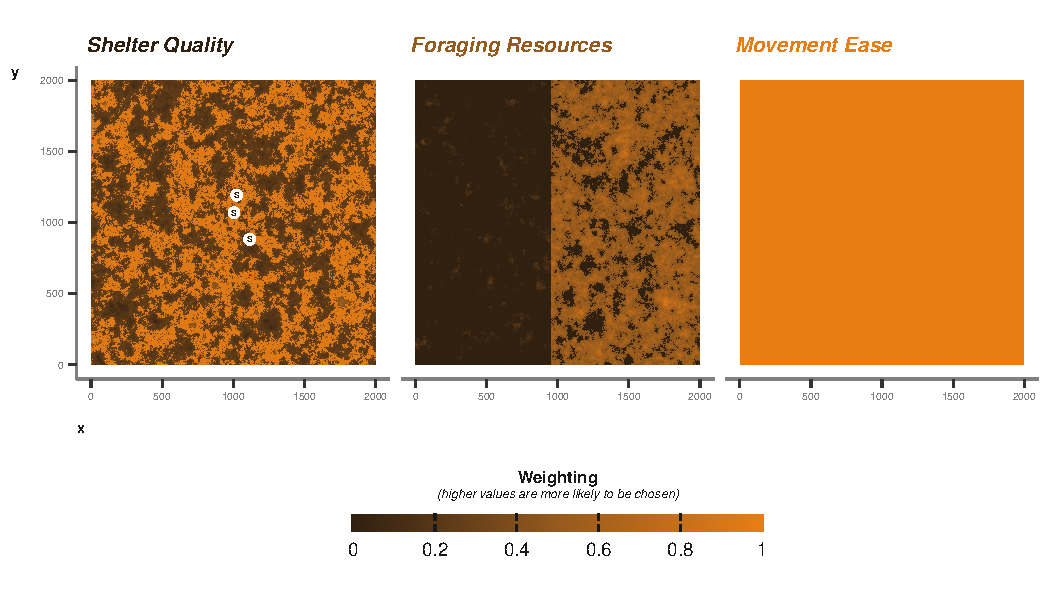
\includegraphics{Agent-based_model_walkthrough_files/figure-latex/VULTURElayersFigure-1} 

}

\caption{The three resulting landscape layers to be fed into the simulation for the vulture example: shelter quality, foraging resources, movement ease.}\label{fig:VULTURElayersFigure}
\end{figure}

\paragraph{King cobra inputs}\label{king-cobra-inputs}

Compared to the vulture, the king cobra movements are smaller, but king cobras can still occupy large areas (Figure \ref{fig:KINGCOBRAmoveCharFigure}).
We provide a rescale value of 10 m to provide a large enough landscape to capture a potentially large range.
The activity cycle provides an opportunity to demonstrate three additive cycles.
The diel cycle is largely similar to the other examples, but we also define an approximately weekly cycle to cover the forage-digestion cycle as well as weak seasonal cycle.
Combined the three cycles create an activity pattern quite different from either the badger or vulture.
To balance the three cycles and their influence on the behaviour transitions, we make some minor adjustments to the underlying behavioural transition matrix.
As mentioned in the ecology and objectives, we want to simulate a barrier limiting movement.
We construct this by altering the values in the environmental matrices, minimising the weighting in cells following two perpendicular lines (Figure \ref{fig:KINGCOBRAlayersFigure}).
We also provide a set of avoidance locations and a relatively weak avoidance weighting coefficient.
Finally, we can set the shelter sites.
We draw 12 sites randomly based on shelter site quality, and limit the area that they can be drawn from to ensure they are not on the far side of the barrier.
We use a larger shelter site size, as king cobras are known to occupy large rock complexes at times.

\begin{Shaded}
\begin{Highlighting}[]
\CommentTok{\# parameters defining Gamma (step length) and Von Mises (turn angle) for each}
\CommentTok{\# behaviour state}
\CommentTok{\# Gamma shape}
\NormalTok{KINGCOBRA\_k\_step }\OtherTok{\textless{}{-}} \FunctionTok{c}\NormalTok{(}\DecValTok{30}\NormalTok{, }\DecValTok{40}\NormalTok{, }\DecValTok{20}\NormalTok{)}
\CommentTok{\# Gamma scale}
\NormalTok{KINGCOBRA\_s\_step }\OtherTok{\textless{}{-}} \FunctionTok{c}\NormalTok{(}\FloatTok{0.75}\NormalTok{, }\FloatTok{1.2}\NormalTok{, }\FloatTok{1.75}\NormalTok{)}
\CommentTok{\# Von Mises mean}
\NormalTok{KINGCOBRA\_mu\_angle }\OtherTok{\textless{}{-}} \FunctionTok{c}\NormalTok{(}\DecValTok{0}\NormalTok{, }\DecValTok{0}\NormalTok{, }\DecValTok{0}\NormalTok{)}
\CommentTok{\# Von Mises concentration}
\NormalTok{KINGCOBRA\_k\_angle }\OtherTok{\textless{}{-}} \FunctionTok{c}\NormalTok{(}\FloatTok{0.6}\NormalTok{, }\FloatTok{0.99}\NormalTok{, }\FloatTok{0.6}\NormalTok{)}

\CommentTok{\# parameters defining Gamma (shape and scale) and Von Mises (mean and}
\CommentTok{\# concentration) for foraging destination options}
\NormalTok{KINGCOBRA\_destinationRange }\OtherTok{\textless{}{-}} \FunctionTok{c}\NormalTok{(}\DecValTok{50}\NormalTok{, }\DecValTok{10}\NormalTok{)}
\NormalTok{KINGCOBRA\_destinationDirection }\OtherTok{\textless{}{-}} \FunctionTok{c}\NormalTok{(}\DecValTok{0}\NormalTok{, }\FloatTok{0.01}\NormalTok{)}
\CommentTok{\# the transformation (2 = squared) and strength of attraction to destinations}
\NormalTok{KINGCOBRA\_destinationTransformation }\OtherTok{\textless{}{-}} \DecValTok{2}
\NormalTok{KINGCOBRA\_destinationModifier }\OtherTok{\textless{}{-}} \FloatTok{1.5}

\CommentTok{\# each cell of the environmental matrix is 10x10}
\NormalTok{KINGCOBRA\_rescale }\OtherTok{\textless{}{-}} \DecValTok{10}

\CommentTok{\# the diel resting/active cycle: amplitude, midline, offset, frequency}
\NormalTok{KINGCOBRA\_rest\_Cycle }\OtherTok{\textless{}{-}} \FunctionTok{c}\NormalTok{(}\FloatTok{0.14}\NormalTok{, }\DecValTok{0}\NormalTok{, }\DecValTok{24}\NormalTok{, }\DecValTok{24}\NormalTok{)}
\CommentTok{\# additional cycles as a dataframe: amplitude, midline, offset, frequency}
\NormalTok{c0 }\OtherTok{\textless{}{-}} \FunctionTok{c}\NormalTok{(}\FloatTok{0.12}\NormalTok{, }\DecValTok{0}\NormalTok{, }\DecValTok{24}\NormalTok{, }\DecValTok{24}\SpecialCharTok{*}\DecValTok{4}\NormalTok{) }\CommentTok{\# digestion}
\NormalTok{c1 }\OtherTok{\textless{}{-}} \FunctionTok{c}\NormalTok{(}\FloatTok{0.05}\NormalTok{, }\DecValTok{0}\NormalTok{, }\DecValTok{24} \SpecialCharTok{*}\NormalTok{ (}\DecValTok{365}\SpecialCharTok{/}\DecValTok{2}\NormalTok{), }\DecValTok{24}\SpecialCharTok{*} \DecValTok{365}\NormalTok{ ) }\CommentTok{\# seasonal}
\NormalTok{KINGCOBRA\_additional\_Cycles }\OtherTok{\textless{}{-}} \FunctionTok{rbind}\NormalTok{(c0, c1)}

\CommentTok{\# select modifications to the default behavioural transition matrix}
\NormalTok{KINGCOBRA\_behaveMatrix }\OtherTok{\textless{}{-}}\NormalTok{ Default\_behaveMatrix}
\NormalTok{KINGCOBRA\_behaveMatrix[}\DecValTok{1}\NormalTok{,}\DecValTok{1}\NormalTok{] }\OtherTok{\textless{}{-}} \FloatTok{0.95}
\NormalTok{KINGCOBRA\_behaveMatrix[}\DecValTok{1}\NormalTok{,}\DecValTok{2}\NormalTok{] }\OtherTok{\textless{}{-}} \FloatTok{0.005}
\NormalTok{KINGCOBRA\_behaveMatrix[}\DecValTok{3}\NormalTok{,}\DecValTok{1}\NormalTok{] }\OtherTok{\textless{}{-}} \FloatTok{0.00025}
\NormalTok{KINGCOBRA\_behaveMatrix[}\DecValTok{3}\NormalTok{,}\DecValTok{2}\NormalTok{] }\OtherTok{\textless{}{-}} \FloatTok{0.000001}
\NormalTok{KINGCOBRA\_behaveMatrix[}\DecValTok{3}\NormalTok{,}\DecValTok{3}\NormalTok{] }\OtherTok{\textless{}{-}} \FloatTok{0.999}

\CommentTok{\# extracting the default matrices ready for changes}
\NormalTok{KINGCOBRA\_shelteringMatrix }\OtherTok{\textless{}{-}}\NormalTok{ landscapeLayersList}\SpecialCharTok{$}\NormalTok{shelter}
\NormalTok{KINGCOBRA\_forageMatrix }\OtherTok{\textless{}{-}}\NormalTok{ landscapeLayersList}\SpecialCharTok{$}\NormalTok{forage}
\NormalTok{KINGCOBRA\_movementMatrix }\OtherTok{\textless{}{-}}\NormalTok{ landscapeLayersList}\SpecialCharTok{$}\NormalTok{movement}
\CommentTok{\# defining the start and end of strong intersections hampering movement}
\NormalTok{roadMin\_x }\OtherTok{\textless{}{-}} \DecValTok{1360}
\NormalTok{roadMax\_x }\OtherTok{\textless{}{-}}\NormalTok{ roadMin\_x }\SpecialCharTok{+} \DecValTok{40}
\NormalTok{roadMin\_y }\OtherTok{\textless{}{-}} \DecValTok{660}
\NormalTok{roadMax\_y }\OtherTok{\textless{}{-}}\NormalTok{ roadMin\_y }\SpecialCharTok{+} \DecValTok{40}

\CommentTok{\# applying the change, dramatically reducing the weighting for all matrices}
\NormalTok{KINGCOBRA\_shelteringMatrix[roadMin\_x}\SpecialCharTok{:}\NormalTok{roadMax\_x,}\DecValTok{1}\SpecialCharTok{:}\DecValTok{2000}\NormalTok{] }\OtherTok{\textless{}{-}}
\NormalTok{  KINGCOBRA\_shelteringMatrix[roadMin\_x}\SpecialCharTok{:}\NormalTok{roadMax\_x,}\DecValTok{1}\SpecialCharTok{:}\DecValTok{2000}\NormalTok{] }\SpecialCharTok{{-}} \DecValTok{90}
\NormalTok{KINGCOBRA\_shelteringMatrix[}\DecValTok{1}\SpecialCharTok{:}\DecValTok{2000}\NormalTok{,roadMin\_y}\SpecialCharTok{:}\NormalTok{roadMax\_y] }\OtherTok{\textless{}{-}}
\NormalTok{  KINGCOBRA\_shelteringMatrix[}\DecValTok{1}\SpecialCharTok{:}\DecValTok{2000}\NormalTok{,roadMin\_y}\SpecialCharTok{:}\NormalTok{roadMax\_y] }\SpecialCharTok{{-}} \DecValTok{90}
\NormalTok{KINGCOBRA\_shelteringMatrix[}\SpecialCharTok{!}\NormalTok{KINGCOBRA\_shelteringMatrix }\SpecialCharTok{\textgreater{}=} \SpecialCharTok{{-}}\FloatTok{99.9}\NormalTok{] }\OtherTok{\textless{}{-}} \SpecialCharTok{{-}}\DecValTok{99}

\NormalTok{KINGCOBRA\_forageMatrix[roadMin\_x}\SpecialCharTok{:}\NormalTok{roadMax\_x,}\DecValTok{1}\SpecialCharTok{:}\DecValTok{2000}\NormalTok{] }\OtherTok{\textless{}{-}}
\NormalTok{  KINGCOBRA\_forageMatrix[roadMin\_x}\SpecialCharTok{:}\NormalTok{roadMax\_x,}\DecValTok{1}\SpecialCharTok{:}\DecValTok{2000}\NormalTok{] }\SpecialCharTok{{-}} \DecValTok{90}
\NormalTok{KINGCOBRA\_forageMatrix[}\DecValTok{1}\SpecialCharTok{:}\DecValTok{2000}\NormalTok{,roadMin\_y}\SpecialCharTok{:}\NormalTok{roadMax\_y] }\OtherTok{\textless{}{-}}
\NormalTok{  KINGCOBRA\_forageMatrix[}\DecValTok{1}\SpecialCharTok{:}\DecValTok{2000}\NormalTok{,roadMin\_y}\SpecialCharTok{:}\NormalTok{roadMax\_y] }\SpecialCharTok{{-}} \DecValTok{90}
\NormalTok{KINGCOBRA\_forageMatrix[}\SpecialCharTok{!}\NormalTok{KINGCOBRA\_forageMatrix }\SpecialCharTok{\textgreater{}=} \SpecialCharTok{{-}}\FloatTok{99.9}\NormalTok{] }\OtherTok{\textless{}{-}} \SpecialCharTok{{-}}\DecValTok{99}

\NormalTok{KINGCOBRA\_movementMatrix[roadMin\_x}\SpecialCharTok{:}\NormalTok{roadMax\_x,}\DecValTok{1}\SpecialCharTok{:}\DecValTok{2000}\NormalTok{] }\OtherTok{\textless{}{-}}
\NormalTok{  KINGCOBRA\_movementMatrix[roadMin\_x}\SpecialCharTok{:}\NormalTok{roadMax\_x,}\DecValTok{1}\SpecialCharTok{:}\DecValTok{2000}\NormalTok{] }\SpecialCharTok{{-}} \DecValTok{90}
\NormalTok{KINGCOBRA\_movementMatrix[}\DecValTok{1}\SpecialCharTok{:}\DecValTok{2000}\NormalTok{,roadMin\_y}\SpecialCharTok{:}\NormalTok{roadMax\_y] }\OtherTok{\textless{}{-}}
\NormalTok{  KINGCOBRA\_movementMatrix[}\DecValTok{1}\SpecialCharTok{:}\DecValTok{2000}\NormalTok{,roadMin\_y}\SpecialCharTok{:}\NormalTok{roadMax\_y] }\SpecialCharTok{{-}} \DecValTok{90}
\NormalTok{KINGCOBRA\_movementMatrix[}\SpecialCharTok{!}\NormalTok{KINGCOBRA\_movementMatrix }\SpecialCharTok{\textgreater{}=} \SpecialCharTok{{-}}\FloatTok{99.9}\NormalTok{] }\OtherTok{\textless{}{-}} \SpecialCharTok{{-}}\DecValTok{99}

\CommentTok{\# defining a number of avoidance points}
\NormalTok{KINGCOBRA\_avoidLocs }\OtherTok{\textless{}{-}} \FunctionTok{data.frame}\NormalTok{(}
  \StringTok{"x"} \OtherTok{=} \FunctionTok{c}\NormalTok{(}\DecValTok{552}\NormalTok{, }\DecValTok{1232}\NormalTok{, }\DecValTok{1587}\NormalTok{),}
  \StringTok{"y"} \OtherTok{=} \FunctionTok{c}\NormalTok{(}\DecValTok{789}\NormalTok{, }\DecValTok{975}\NormalTok{, }\DecValTok{1356}\NormalTok{))}
\CommentTok{\# and specifying a weak avoidance of the points }
\NormalTok{KINGCOBRA\_avoidTransformation }\OtherTok{\textless{}{-}} \DecValTok{2}
\NormalTok{KINGCOBRA\_avoidModifier }\OtherTok{\textless{}{-}} \DecValTok{1}

\CommentTok{\# after the matrices have been altered, drawing 12 shelter sites based on shelter quality}
\NormalTok{sampledShelters }\OtherTok{\textless{}{-}} \FunctionTok{sampleRandom}\NormalTok{(}\FunctionTok{raster}\NormalTok{(KINGCOBRA\_shelteringMatrix), }\DecValTok{12}\NormalTok{,}
                                \AttributeTok{ext =} \FunctionTok{extent}\NormalTok{(}\FloatTok{0.35}\NormalTok{, }\FloatTok{0.65}\NormalTok{, }\FloatTok{0.42}\NormalTok{, }\FloatTok{0.65}\NormalTok{), }
                                \AttributeTok{rowcol =} \ConstantTok{TRUE}\NormalTok{)}
\CommentTok{\# and storing those shelter sites as a dataframe ready for the simulation function}
\NormalTok{KINGCOBRA\_shelterLocs }\OtherTok{\textless{}{-}} \FunctionTok{data.frame}\NormalTok{(}
  \StringTok{"x"} \OtherTok{=}\NormalTok{ sampledShelters[,}\DecValTok{2}\NormalTok{],}
  \StringTok{"y"} \OtherTok{=}\NormalTok{ sampledShelters[,}\DecValTok{1}\NormalTok{])}
\CommentTok{\# specifying a larger shelter site radius}
\NormalTok{KINGCOBRA\_shelterSize }\OtherTok{\textless{}{-}} \DecValTok{10}
\end{Highlighting}
\end{Shaded}

\begin{figure}

{\centering 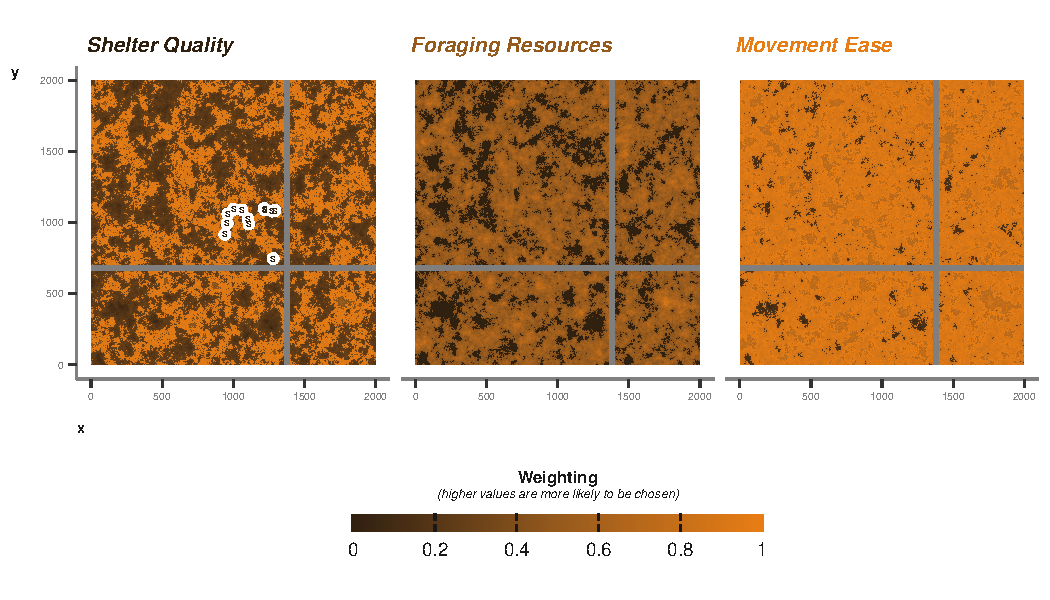
\includegraphics{Agent-based_model_walkthrough_files/figure-latex/KINGCOBRAlayersFigure-1} 

}

\caption{The three resulting landscape layers to be fed into the simulation for the king cobra example: shelter quality, foraging resources, movement ease. Movement ease is blocked by bars of -99 weighting.}\label{fig:KINGCOBRAlayersFigure}
\end{figure}

\clearpage

\subsubsection{Simulation outputs}\label{simulation-outputs}

Figures \ref{fig:VULTUREmoveCharFigure} and \ref{fig:KINGCOBRAmoveCharFigure} describe the inputs for the vulture and king cobra example respectively, and can be compared to the realised movements.
Figures \ref{fig:VULTUREmoveCharFigure}, and \ref{fig:KINGCOBRAmoveCharFigure} also provide information on the rates of stationary behaviour, defined in the plot as step lengths less than the shelter site size.
The king cobra example in particular highlights the prolonged near weekly resting periods.

\begin{figure}

{\centering 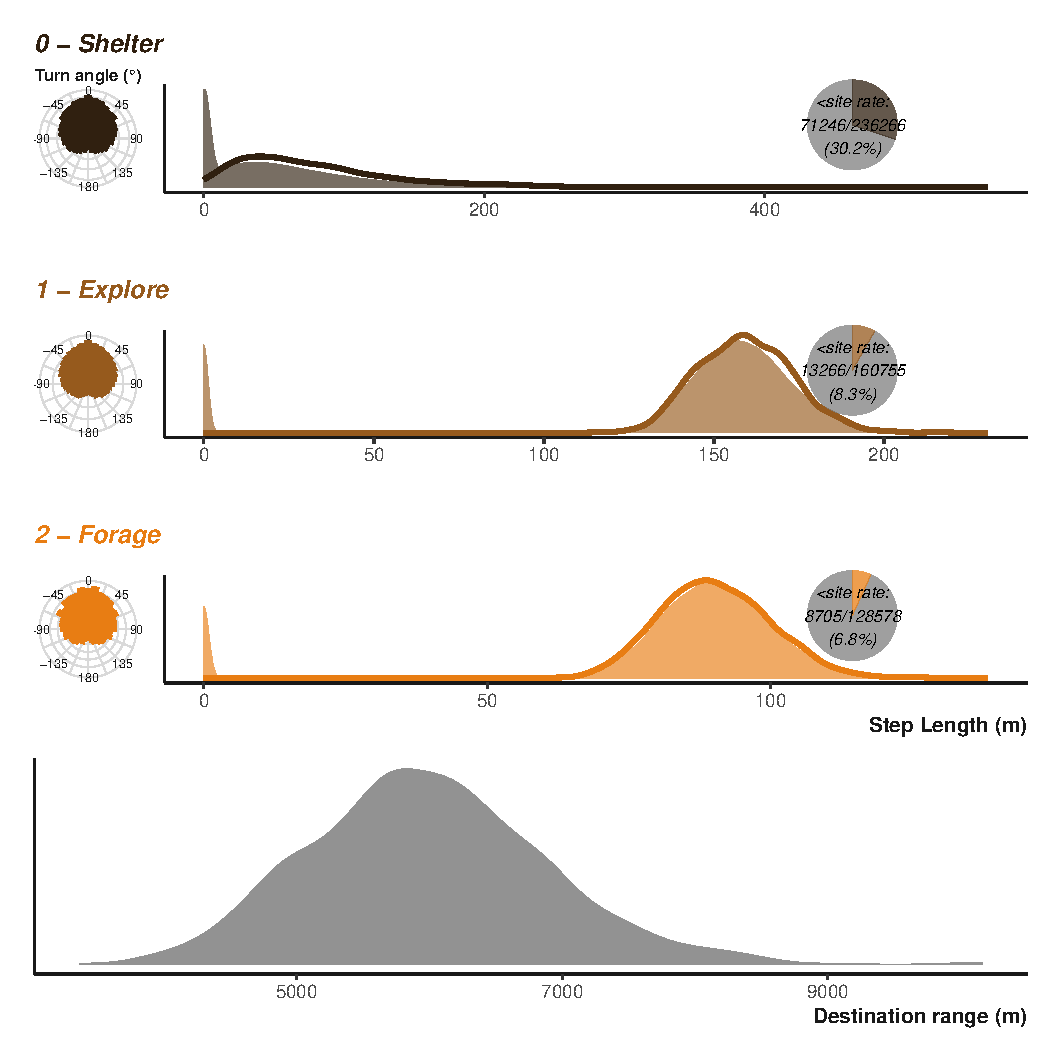
\includegraphics{Agent-based_model_walkthrough_files/figure-latex/VULTUREmoveCharFigure-1} 

}

\caption{The distribution of step lengths used during the vulture simulation example. Parametrising distributions are shown as solid areas using the same shape and scale parameters used as input into the simulation function. The lower plot shows the distribution used to generate potential foraging destinations. The realised resulting simulated step lengths (scaled to the input units) are shown by the solid lines. The realised resulting turn angles are shown in left hand sub-plots. Inset pie charts show the number of step lengths that were below the shelter site size. Note that x axis is not consistent between the three plots.}\label{fig:VULTUREmoveCharFigure}
\end{figure}

\begin{figure}

{\centering 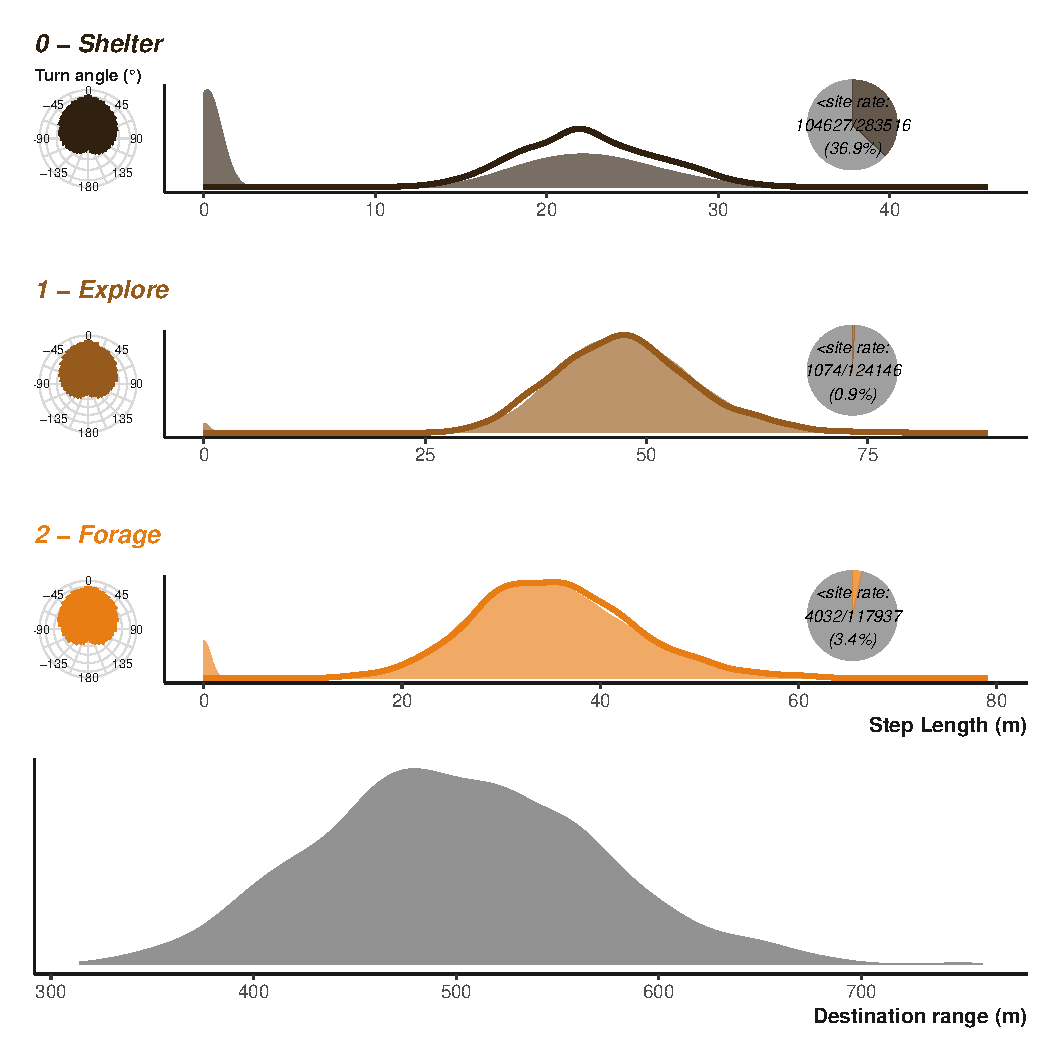
\includegraphics{Agent-based_model_walkthrough_files/figure-latex/KINGCOBRAmoveCharFigure-1} 

}

\caption{The distribution of step lengths used during the king cobra simulation example. Parametrising distributions are shown as solid areas using the same shape and scale parameters used as input into the simulation function. The lower plot shows the distribution used to generate potential foraging destinations. The realised resulting simulated step lengths (scaled to the input units) are shown by the solid lines. The realised resulting turn angles are shown in left hand sub-plots. Inset pie charts show the number of step lengths that were below the shelter site size. Note that x axis is not consistent between the three plots.}\label{fig:KINGCOBRAmoveCharFigure}
\end{figure}

\clearpage

\section{Data availability}\label{data-availability}

All data underlying the results are generated as part of the article, no source data are required.

The example badger, vulture, and king cobra data simulated for this manuscript are available on Zenodo: ``Simulated data from abmAnimalMovement: An R package for simulating animal movement using an agent-based model'' \url{https://doi.org/10.5281/zenodo.6992496}. Files include:

\begin{itemize}
\item
  BADGER\_locations.csv: A csv file that contains the realised locations of the example badger simulation, where each row is equal to a timestep. Columns include: timestep, the timestep as an integer; x, the x coordinate of the animal; y, the y coordinate of the animal; sl, the step length between locations used during the simulation; sl\_rescale the rescale factor required to return step lengths back to the input scale; ta, turning angle between locations in degrees; behave, the behavioural mode the animal was in at a given timestep; chosen, the location chosen out of the number of options available; destination\_x and destination\_y the point the animal was attracted to at that time (note exploratory behaviour is not subject attraction).
\item
  BADGER\_options.csv: A csv file that contains the options available to the example badger simulation over the entire simulation duration, where each row is equal to an option repeated for each timestep. Columns include: timestep, the timestep as an integer; oall\_x, and oall\_y show the x and y coordinates of all the options available to an animal at a timestep; oall\_steplengths are the step lengths from the current location compared to all the options.
\item
  completelist.RDS: This RDS file contains a list object of length three, where the full simulation outputs from each three examples are stored. Each species slot contains the ``locations'' dataframe (see description of locations.csv), the ``options'' dataframe (see description of options.csv), and a nested list containing all the ``inputs'' used to generate the simulated results (split into subsections: inputs\_basic that contains inputs linked to simulation duration and intensity, inputs\_destination that contains inputs linked to destination and attraction aspects, inputs\_movement that contains inputs linked to movement capacity and behavioural switching, inputs\_cycle that contains inputs linked to activity cycling, inputs\_layerSeed that contains the environmental matrices and seed). A fourth object is returned called ``others'' that captures all other outputs, mainly used internally for debugging and checking.
\item
  KINGCOBRA\_locations.csv: A csv file that contains the realised locations of the example king cobra simulation, where each row is equal to a timestep. The file structure follows the same as the BADGER\_options.csv file.
  KINGCOBRA\_options.csv: A csv file that contains the options available to the example king cobra simulation over the entire simulation duration, where each row is equal to an option repeated for each timestep. The file structure follows the same as the BADGER\_options.csv file.
\item
  VULTURE\_locations.csv: A csv file that contains the realised locations of the example vulture simulation, where each row is equal to a timestep. The file structure follows the same as the BADGER\_locations.csv file.
  VULTURE\_options.csv: A csv file that contains the options available to the example vulture simulation over the entire simulation duration, where each row is equal to an option repeated for each timestep. The file structure follows the same as the BADGER\_locations.csv file.
\end{itemize}

Source code to reproduce the results and manuscript are available alongside the software, archived at: \url{https://doi.org/10.5281/zenodo.6951937}.

The parameters used to generate the examples are within: \texttt{notebook/manuscript/Agent-based\_model\_walkthrough.Rmd}.

\section{Software availability}\label{software-availability}

Archived versions of the software are available on Zenodo: ``BenMMarshall/abmAnimalMovement'' \url{https://doi.org/10.5281/zenodo.6951937}.

The development version of the package can be found at \href{https://github.com/BenMMarshall/abmAnimalMovement}{BenMMarshall/abmAnimalMovement}.

License: GPL (\textgreater= 3)

\section{Competing interests}\label{competing-interests}

No competing interests were disclosed.

\section{Grant information}\label{grant-information}

BMM was funded by the Natural Environment Research Council (NERC) via the IAPETUS2 Doctoral Training Partnership.

\section{Author contributions}\label{author-contributions}

Conceptualization: BMM;
Software: BMM;
Supervision: ABD;
Visualization: BMM;
Writing - Original Draft: BMM;
Writing - Review \& Editing: BMM, ABD.

\clearpage

\section*{References}\label{references}
\addcontentsline{toc}{section}{References}

\phantomsection\label{refs}
\begin{CSLReferences}{0}{1}
\bibitem[\citeproctext]{ref-Bastille-Rousseau2017}
\CSLLeftMargin{1. }%
\CSLRightInline{Bastille-Rousseau G, Murray DL, Schaefer JA, Lewis MA, Mahoney SP, Potts JR. \href{https://doi.org/10.1111/ecog.02655}{Spatial scales of habitat selection decisions: {Implications} for telemetry-based movement modelling}. Ecography. 2017;40:1--7. }

\bibitem[\citeproctext]{ref-sridhar_geometry_2021}
\CSLLeftMargin{2. }%
\CSLRightInline{Sridhar VH, Li L, Gorbonos D, Nagy M, Schell BR, Sorochkin T, et al. The geometry of decision-making in individuals and collectives. Proceedings of the National Academy of Sciences {[}Internet{]}. 2021 Dec {[}cited 2022 May 3{]};118(50):e2102157118. Available from: \url{https://pnas.org/doi/full/10.1073/pnas.2102157118}}

\bibitem[\citeproctext]{ref-prange_influences_2004}
\CSLLeftMargin{3. }%
\CSLRightInline{Prange S, Gehrt SD, Wiggers EP. Influences of anthropogenic resources on raccoon ({Procyon} lotor) movements and spatial distribution. Journal of Mammalogy. 2004;85(3):8. }

\bibitem[\citeproctext]{ref-christy_experimental_2017}
\CSLLeftMargin{4. }%
\CSLRightInline{Christy M, Savidge J, Yackel Adams A, Gragg J, Rodda G. Experimental landscape reduction of wild rodents increases movements in the invasive brown treesnake ({Boiga} irregularis). Management of Biological Invasions {[}Internet{]}. 2017 {[}cited 2021 Aug 22{]};8(4):455--67. Available from: \url{http://www.reabic.net/journals/mbi/2017/Issue4.aspx}}

\bibitem[\citeproctext]{ref-vogt_suitability_2018}
\CSLLeftMargin{5. }%
\CSLRightInline{Vogt K, Vimercati E, Ryser A, Hofer E, Signer S, Signer C, et al. Suitability of {GPS} telemetry for studying the predation of {Eurasian} lynx on small- and medium-sized prey animals in the {Northwestern} {Swiss} {Alps}. European Journal of Wildlife Research {[}Internet{]}. 2018 Dec {[}cited 2020 Mar 13{]};64(6):73. Available from: \url{http://link.springer.com/10.1007/s10344-018-1225-7}}

\bibitem[\citeproctext]{ref-loveridge_landscape_2017}
\CSLLeftMargin{6. }%
\CSLRightInline{Loveridge AJ, Valeix M, Elliot NB, Macdonald DW. The landscape of anthropogenic mortality: How {African} lions respond to spatial variation in risk. Howe C, editor. Journal of Applied Ecology {[}Internet{]}. 2017 Jun {[}cited 2019 Jun 4{]};54(3):815--25. Available from: \url{http://doi.wiley.com/10.1111/1365-2664.12794}}

\bibitem[\citeproctext]{ref-Tucker2018}
\CSLLeftMargin{7. }%
\CSLRightInline{Tucker MA, Böhning-Gaese K, Fagan WF, Fryxell JM, Van Moorter B, Alberts SC, et al. Moving in the {Anthropocene}: {Global} reductions in terrestrial mammalian movements. Science {[}Internet{]}. 2018 Jan;359(6374):466--9. Available from: \url{http://www.sciencemag.org/lookup/doi/10.1126/science.aam9712}}

\bibitem[\citeproctext]{ref-tucker_large_2019}
\CSLLeftMargin{8. }%
\CSLRightInline{Tucker MA, Alexandrou O, Bierregaard RO, Bildstein KL, Böhning‐Gaese K, Bracis C, et al. Large birds travel farther in homogeneous environments. Boucher-Lalonde V, editor. Global Ecology and Biogeography {[}Internet{]}. 2019 May {[}cited 2019 May 6{]};28(5):576--87. Available from: \url{https://onlinelibrary.wiley.com/doi/abs/10.1111/geb.12875}}

\bibitem[\citeproctext]{ref-arrondo_invisible_2018}
\CSLLeftMargin{9. }%
\CSLRightInline{Arrondo E, Moleón M, Cortés-Avizanda A, Jiménez J, Beja P, Sánchez-Zapata JA, et al. Invisible barriers: {Differential} sanitary regulations constrain vulture movements across country borders. Biological Conservation {[}Internet{]}. 2018 Mar {[}cited 2022 May 25{]};219:46--52. Available from: \url{https://linkinghub.elsevier.com/retrieve/pii/S0006320717315550}}

\bibitem[\citeproctext]{ref-Fraser2018}
\CSLLeftMargin{10. }%
\CSLRightInline{Fraser KC, Davies KT, Davy CM, Ford AT, Flockhart DTT, Martins EG. Tracking the conservation promise of movement ecology. Frontiers in Ecology and Evolution {[}Internet{]}. 2018;6(October):150. Available from: \url{https://www.frontiersin.org/articles/10.3389/fevo.2018.00150/full?utm_source=F-NTF&utm_medium=EMLX&utm_campaign=PRD_FEOPS_20170000_ARTICLE}}

\bibitem[\citeproctext]{ref-noonan_effects_2020}
\CSLLeftMargin{11. }%
\CSLRightInline{Noonan MJ, Fleming CH, Tucker MA, Kays R, Harrison A, Crofoot MC, et al. Effects of body size on estimation of mammalian area requirements. Conservation Biology {[}Internet{]}. 2020 Jun {[}cited 2020 Jun 23{]};cobi.13495. Available from: \url{https://onlinelibrary.wiley.com/doi/abs/10.1111/cobi.13495}}

\bibitem[\citeproctext]{ref-studd_purrfect_2021}
\CSLLeftMargin{12. }%
\CSLRightInline{Studd EK, Derbyshire RE, Menzies AK, Simms JF, Humphries MM, Murray DL, et al. The {Purr}‐fect {Catch}: {Using} accelerometers and audio recorders to document kill rates and hunting behaviour of a small prey specialist. Methods in Ecology and Evolution {[}Internet{]}. 2021 Jul {[}cited 2022 May 25{]};12(7):1277--87. Available from: \url{https://onlinelibrary.wiley.com/doi/10.1111/2041-210X.13605}}

\bibitem[\citeproctext]{ref-joo_recent_2022}
\CSLLeftMargin{13. }%
\CSLRightInline{Joo R, Picardi S, Boone ME, Clay TA, Patrick SC, Romero-Romero VS, et al. Recent trends in movement ecology of animals and human mobility. Movement Ecology {[}Internet{]}. 2022 May {[}cited 2022 Jun 3{]};10(1):26. Available from: \url{https://doi.org/10.1186/s40462-022-00322-9}}

\bibitem[\citeproctext]{ref-wild_internet_2022}
\CSLLeftMargin{14. }%
\CSLRightInline{Wild TA, Wikelski M, Tyndel S, Alarcón‐Nieto G, Klump BC, Aplin LM, et al. Internet on animals: {Wi}‐{Fi}‐enabled devices provide a solution for big data transmission in biologging. Methods in Ecology and Evolution {[}Internet{]}. 2022 Jan {[}cited 2022 May 25{]};2041--210X.13798. Available from: \url{https://onlinelibrary.wiley.com/doi/10.1111/2041-210X.13798}}

\bibitem[\citeproctext]{ref-kays_movebank_2022}
\CSLLeftMargin{15. }%
\CSLRightInline{Kays R, Davidson SC, Berger M, Bohrer G, Fiedler W, Flack A, et al. The {Movebank} system for studying global animal movement and demography. Methods in Ecology and Evolution {[}Internet{]}. 2022 Feb {[}cited 2022 May 25{]};13(2):419--31. Available from: \url{https://onlinelibrary.wiley.com/doi/10.1111/2041-210X.13767}}

\bibitem[\citeproctext]{ref-saunders_radio-tracking_2022}
\CSLLeftMargin{16. }%
\CSLRightInline{Saunders D, Nguyen H, Cowen S, Magrath M, Marsh K, Bell S, et al. Radio-tracking wildlife with drones: A viewshed analysis quantifying survey coverage across diverse landscapes. Wildlife Research {[}Internet{]}. 2022 Feb {[}cited 2022 May 25{]};49(1):1--10. Available from: \url{https://www.publish.csiro.au/WR/WR21033}}

\bibitem[\citeproctext]{ref-Weatherhead2004}
\CSLLeftMargin{17. }%
\CSLRightInline{Weatherhead PJ, Blouin-Demers G. Long-term effects of radiotelemetry on black ratsnakes. Wildlife Society Bulletin {[}Internet{]}. 2004;32(3):900--6. Available from: \url{http://www.ncbi.nlm.nih.gov/entrez/query.fcgi?db=pubmed&cmd=Retrieve&dopt=AbstractPlus&list_uids=000224767400031}}

\bibitem[\citeproctext]{ref-robstad_impact_2021}
\CSLLeftMargin{18. }%
\CSLRightInline{Robstad CA, Lodberg-Holm HK, Mayer M, Rosell F. The impact of bio-logging on body weight change of the {Eurasian} beaver. PLOS ONE {[}Internet{]}. 2021 Dec {[}cited 2022 May 3{]};16(12):e0261453. Available from: \url{https://journals.plos.org/plosone/article?id=10.1371/journal.pone.0261453}}

\bibitem[\citeproctext]{ref-portugal_externally_2022}
\CSLLeftMargin{19. }%
\CSLRightInline{Portugal SJ, White CR. Externally attached biologgers cause compensatory body mass loss in birds. Methods in Ecology and Evolution {[}Internet{]}. 2022 {[}cited 2022 May 3{]};13(2):294--302. Available from: \url{https://onlinelibrary.wiley.com/doi/abs/10.1111/2041-210X.13754}}

\bibitem[\citeproctext]{ref-clark_ocean_2020}
\CSLLeftMargin{20. }%
\CSLRightInline{Clark TD, Raby GD, Roche DG, Binning SA, Speers-Roesch B, Jutfelt F, et al. Ocean acidification does not impair the behaviour of coral reef fishes. Nature {[}Internet{]}. 2020 Jan {[}cited 2020 Jul 21{]};577(7790):370--5. Available from: \url{http://www.nature.com/articles/s41586-019-1903-y}}

\bibitem[\citeproctext]{ref-roche_behavioural_2020}
\CSLLeftMargin{21. }%
\CSLRightInline{Roche DG, Amcoff M, Morgan R, Sundin J, Finnøen MH, Lawrence MJ, et al. Behavioural lateralisation in a detour test is not repeatable in fishes. EcoEvoRxiv {[}Internet{]}. 2020;62. Available from: \url{https://ecoevorxiv.org/6kcwa}}

\bibitem[\citeproctext]{ref-sanchez-tojar_meta-analysis_2018}
\CSLLeftMargin{22. }%
\CSLRightInline{Sánchez-Tójar A, Nakagawa S, Sánchez-Fortún M, Martin DA, Ramani S, Girndt A, et al. Meta-analysis challenges a textbook example of status signalling and demonstrates publication bias. eLife {[}Internet{]}. 2018 Nov {[}cited 2020 Jul 21{]};7:e37385. Available from: \url{https://elifesciences.org/articles/37385}}

\bibitem[\citeproctext]{ref-wang_irreproducible_2018}
\CSLLeftMargin{23. }%
\CSLRightInline{Wang D, Forstmeier W, Ihle M, Khadraoui M, Jerónimo S, Martin K, et al. Irreproducible text-book {``knowledge''}: {The} effects of color bands on zebra finch fitness: {COLOR} {BANDS} {HAVE} {NO} {EFFECT} {ON} {FITNESS} {IN} {ZEBRA} {FINCHES}. Evolution {[}Internet{]}. 2018 Apr {[}cited 2020 Jul 21{]};72(4):961--76. Available from: \url{http://doi.wiley.com/10.1111/evo.13459}}

\bibitem[\citeproctext]{ref-fraser_role_2020}
\CSLLeftMargin{24. }%
\CSLRightInline{Fraser H, Barnett A, Parker TH, Fidler F. The role of replication studies in ecology. Ecology and Evolution {[}Internet{]}. 2020 Jun {[}cited 2021 Oct 12{]};10(12):5197--207. Available from: \url{https://onlinelibrary.wiley.com/doi/10.1002/ece3.6330}}

\bibitem[\citeproctext]{ref-crane_lots_2021}
\CSLLeftMargin{25. }%
\CSLRightInline{Crane M, Silva I, Marshall BM, Strine CT. Lots of movement, little progress: A review of reptile home range literature. PeerJ {[}Internet{]}. 2021 Jul {[}cited 2021 Jul 20{]};9:e11742. Available from: \url{https://peerj.com/articles/11742}}

\bibitem[\citeproctext]{ref-tam_quantifying_2021}
\CSLLeftMargin{26. }%
\CSLRightInline{Tam J, Lagisz M, Cornwell WK, Nakagawa S. Quantifying research interests in 7,521 mammalian species with h-index: A case study. EcoEvoRxiv {[}Internet{]}. 2021 Nov {[}cited 2022 May 25{]}; Available from: \url{https://osf.io/gd7cv}}

\bibitem[\citeproctext]{ref-williams_optimizing_2020}
\CSLLeftMargin{27. }%
\CSLRightInline{Williams HJ, Taylor LA, Benhamou S, Bijleveld AI, Clay TA, Grissac S, et al. Optimizing the use of biologgers for movement ecology research. Gaillard J, editor. Journal of Animal Ecology {[}Internet{]}. 2020 Jan {[}cited 2020 Jan 31{]};89(1):186--206. Available from: \url{https://onlinelibrary.wiley.com/doi/abs/10.1111/1365-2656.13094}}

\bibitem[\citeproctext]{ref-christie_simple_2019}
\CSLLeftMargin{28. }%
\CSLRightInline{Christie AP, Amano T, Martin PA, Shackelford GE, Simmons BI, Sutherland WJ. Simple study designs in ecology produce inaccurate estimates of biodiversity responses. Journal of Applied Ecology {[}Internet{]}. 2019 {[}cited 2022 May 3{]};56(12):2742--54. Available from: \url{https://onlinelibrary.wiley.com/doi/abs/10.1111/1365-2664.13499}}

\bibitem[\citeproctext]{ref-gupta_reserve_2019}
\CSLLeftMargin{29. }%
\CSLRightInline{Gupta A, Dilkina B, Morin DJ, Fuller AK, Royle JA, Sutherland C, et al. Reserve design to optimize functional connectivity and animal density. Conservation Biology {[}Internet{]}. 2019 Jul {[}cited 2019 Jul 13{]};cobi.13369. Available from: \url{https://onlinelibrary.wiley.com/doi/abs/10.1111/cobi.13369}}

\bibitem[\citeproctext]{ref-debruine_understanding_2021}
\CSLLeftMargin{30. }%
\CSLRightInline{DeBruine LM, Barr DJ. Understanding {Mixed}-{Effects} {Models} {Through} {Data} {Simulation}. Advances in Methods and Practices in Psychological Science. 2021;4(1):1--15. }

\bibitem[\citeproctext]{ref-Sciaini2018}
\CSLLeftMargin{31. }%
\CSLRightInline{Sciaini M, Fritsch M, Scherer C, Simpkins CE. {NLMR} and landscapetools : {An} integrated environment for simulating and modifying neutral landscape models in {R}. Golding N, editor. Methods in Ecology and Evolution {[}Internet{]}. 2018 Nov;9(11):2240--8. Available from: \url{http://doi.wiley.com/10.1111/2041-210X.13076}}

\bibitem[\citeproctext]{ref-petr_slendr_2022}
\CSLLeftMargin{32. }%
\CSLRightInline{Petr M, Haller BC, Ralph PL, Racimo F. Slendr: A framework for spatio-temporal population genomic simulations on geographic landscapes {[}Internet{]}. bioRxiv; 2022 {[}cited 2022 May 3{]}. Available from: \url{https://www.biorxiv.org/content/10.1101/2022.03.20.485041v1}}

\bibitem[\citeproctext]{ref-guerracastro_ssp_2021}
\CSLLeftMargin{33. }%
\CSLRightInline{Guerra‐Castro EJ, Cajas JC, Simões N, Cruz‐Motta JJ, Mascaró M. {SSP}: An {R} package to estimate sampling effort in studies of ecological communities. Ecography {[}Internet{]}. 2021 Apr {[}cited 2022 May 25{]};44(4):561--73. Available from: \url{https://onlinelibrary.wiley.com/doi/10.1111/ecog.05284}}

\bibitem[\citeproctext]{ref-street_solving_2021}
\CSLLeftMargin{34. }%
\CSLRightInline{Street GM, Potts JR, Börger L, Beasley JC, Demarais S, Fryxell JM, et al. Solving the sample size problem for resource selection functions. Methods in Ecology and Evolution {[}Internet{]}. 2021 Dec {[}cited 2022 May 25{]};12(12):2421--31. Available from: \url{https://onlinelibrary.wiley.com/doi/10.1111/2041-210X.13701}}

\bibitem[\citeproctext]{ref-goldstein_integrating_2021}
\CSLLeftMargin{35. }%
\CSLRightInline{Goldstein E, Erinjery JJ, Martin G, Kasturiratne A, Ediriweera DS, Silva HJ de, et al. Integrating human behavior and snake ecology with agent-based models to predict snakebite in high risk landscapes. Habib AG, editor. PLOS Neglected Tropical Diseases {[}Internet{]}. 2021 Jan {[}cited 2022 May 25{]};15(1):e0009047. Available from: \url{https://dx.plos.org/10.1371/journal.pntd.0009047}}

\bibitem[\citeproctext]{ref-Ahearn2001}
\CSLLeftMargin{36. }%
\CSLRightInline{Ahearn SC, Smith JLD, Joshi AR, Ding J. \href{https://doi.org/10.1016/S0304-3800(01)00258-7}{{TIGMOD}: {An} individual-based spatially explicit model for simulating tiger/human interaction in multiple use forests}. Ecological Modelling. 2001 May;140(1-2):81--97. }

\bibitem[\citeproctext]{ref-theng_confronting_2022}
\CSLLeftMargin{37. }%
\CSLRightInline{Theng M, Milleret C, Bracis C, Cassey P, Delean S. Confronting spatial capture--recapture models with realistic animal movement simulations. Ecology {[}Internet{]}. 2022 {[}cited 2022 May 3{]};n/a(n/a):e3676. Available from: \url{https://onlinelibrary.wiley.com/doi/abs/10.1002/ecy.3676}}

\bibitem[\citeproctext]{ref-howe_distance_2017}
\CSLLeftMargin{38. }%
\CSLRightInline{Howe EJ, Buckland ST, Després-Einspenner ML, Kühl HS. Distance sampling with camera traps. Methods in Ecology and Evolution {[}Internet{]}. 2017 {[}cited 2022 May 4{]};8(11):1558--65. Available from: \url{https://onlinelibrary.wiley.com/doi/abs/10.1111/2041-210X.12790}}

\bibitem[\citeproctext]{ref-cappelle_estimating_2021}
\CSLLeftMargin{39. }%
\CSLRightInline{Cappelle N, Howe EJ, Boesch C, Kühl HS. Estimating animal abundance and effort--precision relationship with camera trap distance sampling. Ecosphere {[}Internet{]}. 2021 {[}cited 2022 May 4{]};12(1):e03299. Available from: \url{https://onlinelibrary.wiley.com/doi/abs/10.1002/ecs2.3299}}

\bibitem[\citeproctext]{ref-kellner_two-species_2022}
\CSLLeftMargin{40. }%
\CSLRightInline{Kellner KF, Parsons AW, Kays R, Millspaugh JJ, Rota CT. A {Two}-{Species} {Occupancy} {Model} with a {Continuous}-{Time} {Detection} {Process} {Reveals} {Spatial} and {Temporal} {Interactions}. Journal of Agricultural, Biological and Environmental Statistics {[}Internet{]}. 2022 Jun {[}cited 2022 May 25{]};27(2):321--38. Available from: \url{https://link.springer.com/10.1007/s13253-021-00482-y}}

\bibitem[\citeproctext]{ref-milleret_estimating_2022}
\CSLLeftMargin{41. }%
\CSLRightInline{Milleret C, Dey S, Dupont P, Turek D, Valpine P de, Bischof R. Estimating spatially variable and density-dependent survival using open-population spatial capture-recapture models. bioRxiv {[}Internet{]}. 2022 Mar {[}cited 2022 May 25{]}; Available from: \url{http://biorxiv.org/lookup/doi/10.1101/2022.03.04.482982}}

\bibitem[\citeproctext]{ref-abolaffio_avoiding_2019}
\CSLLeftMargin{42. }%
\CSLRightInline{Abolaffio M, Focardi S, Santini G. Avoiding misleading messages: {Population} assessment using camera trapping is not a simple task. Journal of Animal Ecology {[}Internet{]}. 2019 {[}cited 2022 May 3{]};88(12):2011--6. Available from: \url{https://onlinelibrary.wiley.com/doi/abs/10.1111/1365-2656.13085}}

\bibitem[\citeproctext]{ref-Calabrese2016}
\CSLLeftMargin{43. }%
\CSLRightInline{Calabrese JM, Fleming CH, Gurarie E. \href{https://doi.org/10.1111/2041-210X.12559}{Ctmm: An {R} {Package} for {Analyzing} {Animal} {Relocation} {Data} {As} a {Continuous}-{Time} {Stochastic} {Process}}. Methods in Ecology and Evolution. 2016;7(9):1124--32. }

\bibitem[\citeproctext]{ref-silva_autocorrelationinformed_2022}
\CSLLeftMargin{44. }%
\CSLRightInline{Silva I, Fleming CH, Noonan MJ, Alston J, Folta C, Fagan WF, et al. Autocorrelation‐informed home range estimation: {A} review and practical guide. Methods in Ecology and Evolution {[}Internet{]}. 2022 Mar {[}cited 2022 May 25{]};13(3):534--44. Available from: \url{https://onlinelibrary.wiley.com/doi/10.1111/2041-210X.13786}}

\bibitem[\citeproctext]{ref-Fleming2014}
\CSLLeftMargin{45. }%
\CSLRightInline{Fleming CH, Calabrese JM, Mueller T, Olson KA, Leimgruber P, Fagan WF. From {Fine}-{Scale} {Foraging} to {Home} {Ranges}: {A} {Semivariance} {Approach} to {Identifying} {Movement} {Modes} across {Spatiotemporal} {Scales}. The American Naturalist {[}Internet{]}. 2014;183(5):E154--67. Available from: \url{http://www.jstor.org/stable/10.1086/675504}}

\bibitem[\citeproctext]{ref-Michelot2016}
\CSLLeftMargin{46. }%
\CSLRightInline{Michelot T, Langrock R, Patterson TA. {moveHMM}: An {\textless{}}scp{\textgreater{}}{R}{\textless{}}/scp{\textgreater{}} package for the statistical modelling of animal movement data using hidden {Markov} models. McInerny G, editor. Methods in Ecology and Evolution {[}Internet{]}. 2016 Nov;7(11):1308--15. Available from: \url{http://doi.wiley.com/10.1111/2041-210X.12578}}

\bibitem[\citeproctext]{ref-Tang2010}
\CSLLeftMargin{47. }%
\CSLRightInline{Tang W, Bennett DA. Agent-based {Modeling} of {Animal} {Movement}: {A} {Review}. Geography Compass {[}Internet{]}. 2010 Jul;4(7):682--700. Available from: \url{http://onlinelibrary.wiley.com/doi/10.1111/j.1749-8198.2010.00337.x/full}}

\bibitem[\citeproctext]{ref-quaglietta_simriv_2019}
\CSLLeftMargin{48. }%
\CSLRightInline{Quaglietta L, Porto M. {SiMRiv}: An {R} package for mechanistic simulation of individual, spatially-explicit multistate movements in rivers, heterogeneous and homogeneous spaces incorporating landscape bias. Movement Ecology {[}Internet{]}. 2019 Dec {[}cited 2022 May 25{]};7(1):11. Available from: \url{https://movementecologyjournal.biomedcentral.com/articles/10.1186/s40462-019-0154-8}}

\bibitem[\citeproctext]{ref-VanMoorter2009}
\CSLLeftMargin{49. }%
\CSLRightInline{Van Moorter B, Visscher D, Benhamou S, Börger L, Boyce MS, Gaillard JM. \href{https://doi.org/10.1111/j.1600-0706.2008.17003.x}{Memory keeps you at home: {A} mechanistic model for home range emergence}. Oikos. 2009;118(5):641--52. }

\bibitem[\citeproctext]{ref-bennett_modelling_2006}
\CSLLeftMargin{50. }%
\CSLRightInline{Bennett DA, Tang W. Modelling adaptive, spatially aware, and mobile agents: {Elk} migration in {Yellowstone}. International Journal of Geographical Information Science {[}Internet{]}. 2006 Oct {[}cited 2022 May 25{]};20(9):1039--66. Available from: \url{http://www.tandfonline.com/doi/abs/10.1080/13658810600830806}}

\bibitem[\citeproctext]{ref-Eddelbuettel_seamless_2011}
\CSLLeftMargin{51. }%
\CSLRightInline{Eddelbuettel D, François R. \href{https://doi.org/10.18637/jss.v040.i08}{{Rcpp}: Seamless {R} and {C++} integration}. Journal of Statistical Software. 2011;40(8):1--18. }

\bibitem[\citeproctext]{ref-Eddelbuettel_seamless_2013}
\CSLLeftMargin{52. }%
\CSLRightInline{Eddelbuettel D. \href{https://doi.org/10.1007/978-1-4614-6868-4}{Seamless {R} and {C++} integration with {Rcpp}}. New York: Springer; 2013. }

\bibitem[\citeproctext]{ref-Eddelbuettel_extending_2018}
\CSLLeftMargin{53. }%
\CSLRightInline{Eddelbuettel D, Balamuta JJ. \href{https://doi.org/10.1080/00031305.2017.1375990}{{Extending extit{R} with extit{C++}: A Brief Introduction to extit{Rcpp}}}. The American Statistician. 2018;72(1):28--36. }

\bibitem[\citeproctext]{ref-joo_navigating_2020}
\CSLLeftMargin{54. }%
\CSLRightInline{Joo R, Boone ME, Clay TA, Patrick SC, Clusella‐Trullas S, Basille M. Navigating through the {\textless{}}span style="font-variant:small-caps;"{\textgreater{}}r{\textless{}}/span{\textgreater{}} packages for movement. Börger L, editor. Journal of Animal Ecology {[}Internet{]}. 2020 Jan {[}cited 2021 Aug 29{]};89(1):248--67. Available from: \url{https://onlinelibrary.wiley.com/doi/10.1111/1365-2656.13116}}

\bibitem[\citeproctext]{ref-Nathan2008}
\CSLLeftMargin{55. }%
\CSLRightInline{Nathan R, Getz WM, Revilla E, Holyoak M, Kadmon R, Saltz D, et al. A movement ecology paradigm for unifying organismal movement research. Proceedings of the National Academy of Sciences {[}Internet{]}. 2008;105(49):19052--9. Available from: \url{http://www.pnas.org/content/105/49/19052.abstract}}

\bibitem[\citeproctext]{ref-rivera_rethinking_2022}
\CSLLeftMargin{56. }%
\CSLRightInline{Rivera K, Fidino M, Farris ZJ, Magle SB, Murphy A, Gerber BD. Rethinking habitat occupancy modeling and the role of diel activity in an anthropogenic world. The American Naturalist {[}Internet{]}. 2022 May {[}cited 2022 May 6{]}; Available from: \url{https://www.journals.uchicago.edu/doi/10.1086/720714}}

\bibitem[\citeproctext]{ref-Scharf2018}
\CSLLeftMargin{57. }%
\CSLRightInline{Scharf AK, Belant JL, Beyer DE, Wikelski M, Safi K. Habitat suitability does not capture the essence of animal-defined corridors. Movement Ecology {[}Internet{]}. 2018;6(1):18. Available from: \url{https://movementecologyjournal.biomedcentral.com/articles/10.1186/s40462-018-0136-2}}

\bibitem[\citeproctext]{ref-kowalczyk_daily_2006}
\CSLLeftMargin{58. }%
\CSLRightInline{Kowalczyk R, Zalewski A, Bogumiła J. Daily movement and territory use by badgers {Meles} meles in {Białowieża} {Primeval} {Forest}, {Poland}. Wildlife Biology {[}Internet{]}. 2006 Dec {[}cited 2022 May 26{]};12(4):385--91. Available from: \url{http://www.bioone.org/doi/abs/10.2981/0909-6396\%282006\%2912\%5B385\%3ADMATUB\%5D2.0.CO\%3B2}}

\bibitem[\citeproctext]{ref-feore_habitat_1999}
\CSLLeftMargin{59. }%
\CSLRightInline{Feore S, Montgomery WI. Habitat effects on the spatial ecology of the {European} badger (\emph{{Meles} meles}). Journal of Zoology {[}Internet{]}. 1999 Apr {[}cited 2022 May 26{]};247(4):537--49. Available from: \url{https://onlinelibrary.wiley.com/doi/10.1111/j.1469-7998.1999.tb01015.x}}

\bibitem[\citeproctext]{ref-rosalino_activity_2005}
\CSLLeftMargin{60. }%
\CSLRightInline{Rosalino LM, Macdonald DW, Santos-Reis M. Activity rhythms, movements and patterns of sett use by badgers, {Meles} meles, in a {Mediterranean} woodland. Mammalia {[}Internet{]}. 2005 Jan {[}cited 2022 May 26{]};69(3-4). Available from: \url{https://www.degruyter.com/document/doi/10.1515/mamm.2005.031/html}}

\bibitem[\citeproctext]{ref-kelly_extra_2020}
\CSLLeftMargin{61. }%
\CSLRightInline{Kelly DJ, Gaughran A, Mullen E, MacWhite T, Maher P, Good M, et al. Extra {Territorial} {Excursions} by {European} badgers are not limited by age, sex or season. Scientific Reports {[}Internet{]}. 2020 Dec {[}cited 2022 May 25{]};10(1):9665. Available from: \url{http://www.nature.com/articles/s41598-020-66809-w}}

\bibitem[\citeproctext]{ref-loureiro_path_2007}
\CSLLeftMargin{62. }%
\CSLRightInline{Loureiro F, Rosalino LM, Macdonald DW, Santos-Reis M. Path tortuosity of {Eurasian} badgers ({Meles} meles) in a heterogeneous {Mediterranean} landscape. Ecological Research {[}Internet{]}. 2007 Aug {[}cited 2022 May 26{]};22(5):837--44. Available from: \url{http://doi.wiley.com/10.1007/s11284-006-0325-0}}

\bibitem[\citeproctext]{ref-magowan_dead-reckoning_2022}
\CSLLeftMargin{63. }%
\CSLRightInline{Magowan EA, Maguire IE, Smith S, Redpath S, Marks NJ, Wilson RP, et al. Dead-reckoning elucidates fine-scale habitat use by {European} badgers {Meles} meles. Animal Biotelemetry {[}Internet{]}. 2022 Dec {[}cited 2022 May 26{]};10(1):10. Available from: \url{https://animalbiotelemetry.biomedcentral.com/articles/10.1186/s40317-022-00282-2}}

\bibitem[\citeproctext]{ref-Eddelbuettel_BH_2021}
\CSLLeftMargin{64. }%
\CSLRightInline{Eddelbuettel D, Emerson JW, Kane MJ. BH: Boost c++ header files {[}Internet{]}. 2021. Available from: \url{https://CRAN.R-project.org/package=BH}}

\bibitem[\citeproctext]{ref-R-base}
\CSLLeftMargin{65. }%
\CSLRightInline{R Core Team. R: A language and environment for statistical computing {[}Internet{]}. Vienna, Austria: R Foundation for Statistical Computing; 2021. Available from: \url{https://www.R-project.org/}}

\bibitem[\citeproctext]{ref-Wickham_devtools_2021}
\CSLLeftMargin{66. }%
\CSLRightInline{Wickham H, Hester J, Chang W, Bryan J. Devtools: Tools to make developing r packages easier {[}Internet{]}. 2021. Available from: \url{https://CRAN.R-project.org/package=devtools}}

\bibitem[\citeproctext]{ref-RStudioTeam2021}
\CSLLeftMargin{67. }%
\CSLRightInline{RStudio Team. RStudio: Integrated development environment for r {[}Internet{]}. Boston, MA: RStudio, PBC; 2021. Available from: \url{http://www.rstudio.com/}}

\bibitem[\citeproctext]{ref-R-rmarkdown}
\CSLLeftMargin{68. }%
\CSLRightInline{Allaire J, Xie Y, McPherson J, Luraschi J, Ushey K, Atkins A, et al. Rmarkdown: Dynamic documents for r {[}Internet{]}. 2022. Available from: \url{https://CRAN.R-project.org/package=rmarkdown}}

\bibitem[\citeproctext]{ref-rmarkdown2018}
\CSLLeftMargin{69. }%
\CSLRightInline{Xie Y, Allaire JJ, Grolemund G. R markdown: The definitive guide {[}Internet{]}. Boca Raton, Florida: Chapman; Hall/CRC; 2018. Available from: \url{https://bookdown.org/yihui/rmarkdown}}

\bibitem[\citeproctext]{ref-rmarkdown2020}
\CSLLeftMargin{70. }%
\CSLRightInline{Xie Y, Dervieux C, Riederer E. R markdown cookbook {[}Internet{]}. Boca Raton, Florida: Chapman; Hall/CRC; 2020. Available from: \url{https://bookdown.org/yihui/rmarkdown-cookbook}}

\bibitem[\citeproctext]{ref-bookdown2016}
\CSLLeftMargin{71. }%
\CSLRightInline{Xie Y. Bookdown: Authoring books and technical documents with {R} markdown {[}Internet{]}. Boca Raton, Florida: Chapman; Hall/CRC; 2016. Available from: \url{https://bookdown.org/yihui/bookdown}}

\bibitem[\citeproctext]{ref-R-bookdown}
\CSLLeftMargin{72. }%
\CSLRightInline{Xie Y. Bookdown: Authoring books and technical documents with r markdown {[}Internet{]}. 2022. Available from: \url{https://CRAN.R-project.org/package=bookdown}}

\bibitem[\citeproctext]{ref-tinytex2019}
\CSLLeftMargin{73. }%
\CSLRightInline{Xie Y. TinyTeX: A lightweight, cross-platform, and easy-to-maintain LaTeX distribution based on TeX live. TUGboat {[}Internet{]}. 2019;(1):30--2. Available from: \url{https://tug.org/TUGboat/Contents/contents40-1.html}}

\bibitem[\citeproctext]{ref-R-tinytex}
\CSLLeftMargin{74. }%
\CSLRightInline{Xie Y. Tinytex: Helper functions to install and maintain TeX live, and compile LaTeX documents {[}Internet{]}. 2022. Available from: \url{https://github.com/rstudio/tinytex}}

\bibitem[\citeproctext]{ref-knitr2015}
\CSLLeftMargin{75. }%
\CSLRightInline{Xie Y. Dynamic documents with {R} and knitr {[}Internet{]}. 2nd ed. Boca Raton, Florida: Chapman; Hall/CRC; 2015. Available from: \url{https://yihui.org/knitr/}}

\bibitem[\citeproctext]{ref-knitr2014}
\CSLLeftMargin{76. }%
\CSLRightInline{Xie Y. Knitr: A comprehensive tool for reproducible research in {R}. In: Stodden V, Leisch F, Peng RD, editors. Implementing reproducible computational research {[}Internet{]}. Chapman; Hall/CRC; 2014. Available from: \url{http://www.crcpress.com/product/isbn/9781466561595}}

\bibitem[\citeproctext]{ref-R-knitr}
\CSLLeftMargin{77. }%
\CSLRightInline{Xie Y. Knitr: A general-purpose package for dynamic report generation in r {[}Internet{]}. 2022. Available from: \url{https://yihui.org/knitr/}}

\bibitem[\citeproctext]{ref-R-here}
\CSLLeftMargin{78. }%
\CSLRightInline{Müller K. Here: A simpler way to find your files {[}Internet{]}. 2020. Available from: \url{https://CRAN.R-project.org/package=here}}

\bibitem[\citeproctext]{ref-R-dplyr}
\CSLLeftMargin{79. }%
\CSLRightInline{Wickham H, François R, Henry L, Müller K. Dplyr: A grammar of data manipulation {[}Internet{]}. 2022. Available from: \url{https://CRAN.R-project.org/package=dplyr}}

\bibitem[\citeproctext]{ref-reshape22007}
\CSLLeftMargin{80. }%
\CSLRightInline{Wickham H. Reshaping data with the {reshape} package. Journal of Statistical Software {[}Internet{]}. 2007;21(12):1--20. Available from: \url{http://www.jstatsoft.org/v21/i12/}}

\bibitem[\citeproctext]{ref-R-ggplot2}
\CSLLeftMargin{81. }%
\CSLRightInline{Wickham H, Chang W, Henry L, Pedersen TL, Takahashi K, Wilke C, et al. ggplot2: Create elegant data visualisations using the grammar of graphics {[}Internet{]}. 2022. Available from: \url{https://CRAN.R-project.org/package=ggplot2}}

\bibitem[\citeproctext]{ref-ggplot22016}
\CSLLeftMargin{82. }%
\CSLRightInline{Wickham H. ggplot2: Elegant graphics for data analysis {[}Internet{]}. Springer-Verlag New York; 2016. Available from: \url{https://ggplot2.tidyverse.org}}

\bibitem[\citeproctext]{ref-R-ggridges}
\CSLLeftMargin{83. }%
\CSLRightInline{Wilke CO. Ggridges: Ridgeline plots in ggplot2 {[}Internet{]}. 2021. Available from: \url{https://wilkelab.org/ggridges/}}

\bibitem[\citeproctext]{ref-R-ggtext}
\CSLLeftMargin{84. }%
\CSLRightInline{Wilke CO. Ggtext: Improved text rendering support for ggplot2 {[}Internet{]}. 2020. Available from: \url{https://wilkelab.org/ggtext/}}

\bibitem[\citeproctext]{ref-R-ggforce}
\CSLLeftMargin{85. }%
\CSLRightInline{Pedersen TL. Ggforce: Accelerating ggplot2 {[}Internet{]}. 2021. Available from: \url{https://CRAN.R-project.org/package=ggforce}}

\bibitem[\citeproctext]{ref-R-patchwork}
\CSLLeftMargin{86. }%
\CSLRightInline{Pedersen TL. Patchwork: The composer of plots {[}Internet{]}. 2020. Available from: \url{https://CRAN.R-project.org/package=patchwork}}

\bibitem[\citeproctext]{ref-R-raster}
\CSLLeftMargin{87. }%
\CSLRightInline{Hijmans RJ. Raster: Geographic data analysis and modeling {[}Internet{]}. 2022. Available from: \url{https://rspatial.org/raster}}

\bibitem[\citeproctext]{ref-sp2013}
\CSLLeftMargin{88. }%
\CSLRightInline{Bivand RS, Pebesma E, Gomez-Rubio V. Applied spatial data analysis with {R}, second edition {[}Internet{]}. Springer, NY; 2013. Available from: \url{https://asdar-book.org/}}

\bibitem[\citeproctext]{ref-sp2005}
\CSLLeftMargin{89. }%
\CSLRightInline{Pebesma EJ, Bivand RS. Classes and methods for spatial data in {R}. R News {[}Internet{]}. 2005;5(2):9--13. Available from: \url{https://CRAN.R-project.org/doc/Rnews/}}

\bibitem[\citeproctext]{ref-R-sp}
\CSLLeftMargin{90. }%
\CSLRightInline{Pebesma E, Bivand R. Sp: Classes and methods for spatial data {[}Internet{]}. 2022. Available from: \url{https://CRAN.R-project.org/package=sp}}

\bibitem[\citeproctext]{ref-NLMR2018}
\CSLLeftMargin{91. }%
\CSLRightInline{Sciaini M, Fritsch M, Scherer C, Simpkins CE. NLMR and landscapetools: An integrated environment for simulating and modifying neutral landscape models in r. Methods in Ecololgy and Evolution {[}Internet{]}. 2018;00:1--9. Available from: \url{https://doi.org/10.1111/2041-210X.13076}}

\bibitem[\citeproctext]{ref-R-NLMR}
\CSLLeftMargin{92. }%
\CSLRightInline{Sciaini M, Fritsch M, Hesselbarth M, Simpkins C, Scherer C, Hanß S. NLMR: Simulating neutral landscape models {[}Internet{]}. 2021. Available from: \url{https://ropensci.github.io/NLMR/}}

\bibitem[\citeproctext]{ref-Quintana2020}
\CSLLeftMargin{93. }%
\CSLRightInline{Quintana DS. A synthetic dataset primer for the biobehavioural sciences to promote reproducibility and hypothesis generation. Zaidi M, Büchel C, Bishop DVM, editors. eLife {[}Internet{]}. 2020 Mar;9:e53275. Available from: \url{https://doi.org/10.7554/eLife.53275}}

\bibitem[\citeproctext]{ref-Gerstner2017}
\CSLLeftMargin{94. }%
\CSLRightInline{Gerstner K, Moreno-Mateos D, Gurevitch J, Beckmann M, Kambach S, Jones HP, et al. Will your paper be used in a meta-analysis? Make the reach of your research broader and longer lasting. Methods in Ecology and Evolution {[}Internet{]}. 2017;8(6):777--84. Available from: \url{https://besjournals.onlinelibrary.wiley.com/doi/abs/10.1111/2041-210X.12758}}

\bibitem[\citeproctext]{ref-hribsek_first_2021}
\CSLLeftMargin{95. }%
\CSLRightInline{Hribsek I, Plecas M, Skoric S, Marinkovic S. First description of movement and ranging behavior of the {Griffon} vulture ({Gyps} fulvus) from {Serbia} using {GPS} satellite tracking. Archives of Biological Sciences {[}Internet{]}. 2021 {[}cited 2022 May 25{]};73(2):185--95. Available from: \url{http://www.doiserbia.nb.rs/Article.aspx?ID=0354-46642100013H}}

\bibitem[\citeproctext]{ref-garcia-jimenez_drivers_2018}
\CSLLeftMargin{96. }%
\CSLRightInline{García-Jiménez R, Pérez-García JM, Margalida A. Drivers of daily movement patterns affecting an endangered vulture flight activity. BMC Ecology {[}Internet{]}. 2018 Dec {[}cited 2022 May 25{]};18(1):39. Available from: \url{https://bmcecol.biomedcentral.com/articles/10.1186/s12898-018-0195-7}}

\bibitem[\citeproctext]{ref-margalida_spatial_2016}
\CSLLeftMargin{97. }%
\CSLRightInline{Margalida A, Pérez-García JM, Afonso I, Moreno-Opo R. Spatial and temporal movements in {Pyrenean} bearded vultures ({Gypaetus} barbatus): {Integrating} movement ecology into conservation practice. Scientific Reports {[}Internet{]}. 2016 Dec {[}cited 2022 May 25{]};6(1):35746. Available from: \url{http://www.nature.com/articles/srep35746}}

\bibitem[\citeproctext]{ref-subedi_spatial_2020}
\CSLLeftMargin{98. }%
\CSLRightInline{Subedi TR, Pérez‐García JM, Sah SAM, Gurung S, Baral HS, Poudyal LP, et al. Spatial and temporal movement of the {Bearded} {Vulture} using {GPS} telemetry in the {Himalayas} of {Nepal}. Ibis {[}Internet{]}. 2020 Apr {[}cited 2022 May 25{]};162(2):563--71. Available from: \url{https://onlinelibrary.wiley.com/doi/10.1111/ibi.12799}}

\bibitem[\citeproctext]{ref-bracis_revisitation_2018}
\CSLLeftMargin{99. }%
\CSLRightInline{Bracis C, Bildstein KL, Mueller T. Revisitation analysis uncovers spatio-temporal patterns in animal movement data. Ecography {[}Internet{]}. 2018; Available from: \url{http://dx.doi.org/10.1111/ecog.03618}}

\bibitem[\citeproctext]{ref-silva_seasonal_2017}
\CSLLeftMargin{100. }%
\CSLRightInline{Silva R, Afán I, Gil JA, Bustamante J. Seasonal and circadian biases in bird tracking with solar {GPS}-tags. Margalida A, editor. PLOS ONE {[}Internet{]}. 2017 Oct {[}cited 2022 May 25{]};12(10):e0185344. Available from: \url{https://dx.plos.org/10.1371/journal.pone.0185344}}

\bibitem[\citeproctext]{ref-peshev_new_2021}
\CSLLeftMargin{101. }%
\CSLRightInline{Peshev H, Grozdanov A, Kmetova--Biro E, Ivanov I, Stoyanov G, Tsiakiris R, et al. New insight into spatial ecology of {Griffon} {Vulture} ({Gyps} fulvus) on the {Balkans} provides opportunity for focusing conservation actions for a threatened social scavenger. Biodiversity Data Journal {[}Internet{]}. 2021 Aug {[}cited 2022 May 25{]};9:e71100. Available from: \url{https://bdj.pensoft.net/article/71100/}}

\bibitem[\citeproctext]{ref-Marshall2018}
\CSLLeftMargin{102. }%
\CSLRightInline{Marshall BM, Strine CT, Jones MD, Artchawakom T, Silva I, Suwanwaree P, et al. Space fit for a king: Spatial ecology of king cobras ({Ophiophagus} hannah) in {Sakaerat} {Biosphere} {Reserve}, {Northeastern} {Thailand}. Amphibia-Reptilia {[}Internet{]}. 2019 Mar;40(2):163--78. Available from: \url{http://booksandjournals.brillonline.com/content/journals/10.1163/15685381-18000008}}

\bibitem[\citeproctext]{ref-marshall_no_2020}
\CSLLeftMargin{103. }%
\CSLRightInline{Marshall BM, Crane M, Silva I, Strine CT, Jones MD, Hodges CW, et al. No room to roam: {King} {Cobras} reduce movement in agriculture. Movement Ecology {[}Internet{]}. 2020 Dec {[}cited 2020 Aug 4{]};8(1):33. Available from: \url{https://movementecologyjournal.biomedcentral.com/articles/10.1186/s40462-020-00219-5}}

\bibitem[\citeproctext]{ref-dsouza_space_2021}
\CSLLeftMargin{104. }%
\CSLRightInline{D'souza A, Gale GA, Marshall BM, Khamcha D, Waengsothorn S, Strine CT. Space use and activity of {Boiga} cyanea -- {A} major songbird nest predator in a seasonal tropical forest in {Thailand}. Global Ecology and Conservation {[}Internet{]}. 2021 Dec {[}cited 2021 Oct 27{]};32:e01875. Available from: \url{https://linkinghub.elsevier.com/retrieve/pii/S235198942100425X}}

\bibitem[\citeproctext]{ref-smith_native_2021}
\CSLLeftMargin{105. }%
\CSLRightInline{Smith SN, Jones MD, Marshall BM, Waengsothorn S, Gale GA, Strine CT. Native {Burmese} pythons exhibit site fidelity and preference for aquatic habitats in an agricultural mosaic. Scientific Reports {[}Internet{]}. 2021 Dec {[}cited 2021 Mar 29{]};11(1):7014. Available from: \url{http://www.nature.com/articles/s41598-021-86640-1}}

\bibitem[\citeproctext]{ref-Siers2018}
\CSLLeftMargin{106. }%
\CSLRightInline{Siers SR, Yackel Adams AA, Reed RN. Behavioral differences following ingestion of large meals and consequences for management of a harmful invasive snake: {A} field experiment. Ecology and Evolution {[}Internet{]}. 2018 Oct;8(20):10075--93. Available from: \url{http://doi.wiley.com/10.1002/ece3.4480}}

\bibitem[\citeproctext]{ref-jones_how_2022}
\CSLLeftMargin{107. }%
\CSLRightInline{Jones MD, Marshall BM, Smith SN, Crane M, Silva I, Artchawakom T, et al. How do {King} {Cobras} move across a major highway? {Unintentional} wildlife crossing structures may facilitate movement. Ecology and Evolution {[}Internet{]}. 2022 Mar {[}cited 2022 Mar 21{]};12(3). Available from: \url{https://onlinelibrary.wiley.com/doi/10.1002/ece3.8691}}

\bibitem[\citeproctext]{ref-Marshall2018b}
\CSLLeftMargin{108. }%
\CSLRightInline{Marshall BM, Strine CT, Jones MD, Theodorou A, Amber E, Waengsothorn S, et al. Hits {Close} to {Home}: {Repeated} {Persecution} of {King} {Cobras} ({Ophiophagus} hannah) in {Northeastern} {Thailand}. Tropical Conservation Science {[}Internet{]}. 2018 Jan;11:194008291881840. Available from: \url{http://journals.sagepub.com/doi/10.1177/1940082918818401}}

\bibitem[\citeproctext]{ref-Shankar2013}
\CSLLeftMargin{109. }%
\CSLRightInline{Shankar PG, Ganesh SR, Whitaker R, Prashanth P. King {Cobra} {Ophiophagus} hannah ({Cantor}, 1836) encounters in human-modified rainforests of the {Western} {Ghats}, {India}. Hamadryad. 2013;36(2):62--8. }

\bibitem[\citeproctext]{ref-Silva2018}
\CSLLeftMargin{110. }%
\CSLRightInline{Silva I, Crane M, Suwanwaree P, Strine C, Goode M. Using dynamic {Brownian} {Bridge} {Movement} {Models} to identify home range size and movement patterns in king cobras. Munderloh UG, editor. PLOS ONE {[}Internet{]}. 2018 Sep;13(9):e0203449. Available from: \url{http://dx.plos.org/10.1371/journal.pone.0203449}}

\end{CSLReferences}

\end{document}
